\RequirePackage{fix-cm}
%
%\documentclass{svjour3}                     % onecolumn (standard format)
%\documentclass[smallcondensed]{svjour3}     % onecolumn (ditto)
\documentclass[smallextended]{svjour3}       % onecolumn (second format)
%\documentclass[twocolumn]{svjour3}          % twocolumn
%
\smartqed  % flush right qed marks, e.g. at end of proof
%
\usepackage{graphicx}
\usepackage{color}
\usepackage{url}
\usepackage{multicol}

%
% \usepackage{mathptmx}      % use Times fonts if available on your TeX system
%
% insert here the call for the packages your document requires
%\usepackage{latexsym}
% etc.
%
% please place your own definitions here and don't use \def but
% \newcommand{}{}
%
% Insert the name of "your journal" with
% \journalname{myjournal}
%
\begin{document}

\title{Automated Refactoring of Rust Programs%\thanks{Grants or other notes
%about the article that should go on the front page should be
%placed here. General acknowledgments should be placed at the end of the article.}
}
\subtitle{}% Do you have a subtitle?\\ If so, write it here

%\titlerunning{Short form of title}        % if too long for running head

\author{Garming Sam \and Nick Cameron \and Alex Potanin}

%\authorrunning{Short form of author list} % if too long for running head

\institute{A. Potanin \at
              School of Engineering and Computer Science \\
              Victoria University of Wellingon, New Zealand \\
              \email{alex@ecs.vuw.ac.nz}           %  \\
%             \emph{Present address:} of F. Author  %  if needed
%           \and
%           S. Author \at
%              second address
}

\date{Received: date / Accepted: date}
% The correct dates will be entered by the editor

\maketitle

\begin{abstract}
The purpose of this document is to outline a new automated refactoring tool for the Rust programming language. The creation of the tool serves as an explorative process to investigate the current ability for Rust to provide automated refactorings and to draw comparisons to  efforts in providing refactoring tools for other languages. 

Beginning with a review of refactoring in general and Rust, this document describes an overview of the tool along with a selection of the major design decisions. Elaborating further, technical details and Rust-specifics are explored with respect to the capability and limitations of the tool. Evaluating the tool, the correctness of each refactoring is examined, as well as the practical use of the tool.

Regarding Rust specific aspects of refactoring, a number of further extensions to this tool are proposed, along with extensions to the Rust compiler which would help facilitate this work. In particular, based on evaluation, the issue of efficiency of the tool should be further addressed and streamlining the process for convenient refactoring will contribute to the practical use of the tool.
\keywords{First keyword \and Second keyword \and More}
% \PACS{PACS code1 \and PACS code2 \and more}
% \subclass{MSC code1 \and MSC code2 \and more}
\end{abstract}

\section{Introduction}\label{C:intro}

The Rust programming language reached the 1.0 milestone \cite{rustcore15} back in May 2015. Backed by Mozilla and Mozilla Research, Rust is open source and generates a number of contributions from the community. As a modern memory-safe systems programming language, the aim for the language is to provide reliable and efficient systems by combining the performance of low level control, with the convenience and guarantees of higher level constructs. All of this is achieved without a garbage collector or runtime and allows interoperability with no overhead with C. Rust enforces an ownership system to restrict the duplication of references through borrowing and lifetimes, while still aiming for `zero cost abstractions'. Using these techniques, Rust prevents dangling pointers and a whole class of related issues concerning iterator invalidation, concurrency and more \cite{rustbook15}.

Rust has been a number of years in the making, beginning as a side-project in 2006 \cite{faq15}, but only with this public 1.0 release has many of the standard library API stabilised. In order to further present itself as a stable and mature language, there is still another component which has yet to be adequately tackled: tooling. Developers commonly use a rich set of tools to simplify the task of building complex software with IDE, editors and debuggers. Such tools can improve productivity and providing tools specific to a language may help to encourage adoption.

Refactoring is the act of performing functionality preserving code transformation. Traditionally, these transformations needed to be performed manually, but in recent years, a number of tools to aid and automate refactorings have arisen in many programming languages such as Java or C++ \cite{brown2008tool}. Manual transformations, including editor search-and-replace are potentially prone to error and so performing tool-assisted refactoring which guarantees some measure of correctness can provide much greater confidence in changes.

The main purpose of this work is to produce a proof-of-concept refactoring tool which utilises existing infrastructure made available by the Rust compiler. The idea was to produce a tool which may be run to provide a set of refactorings, which may continue to be extended in the future. The list of implemented refactorings is as follows:

\begin{itemize}
\item {\bfseries Renaming local and global variables} -- Variables declared within a function or method, or in a global namespace
%\item {\bfseries Renaming global variables} -- Variables in a global namespace
\item {\bfseries Renaming function arguments} -- Renaming local variables declared by a function or method signature
\item {\bfseries Renaming fields} -- Struct-local members
\item {\bfseries Renaming functions and methods} -- Statically or dynamically dispatched functions, and functions belonging to objects, including overridden methods
\item {\bfseries Renaming structs} -- Custom data types declaring fields and methods
\item {\bfseries Renaming enumerations} -- Enumerated data types declaring fields and methods
\item {\bfseries Inlining local variables} -- Replacing usages of a local variable with its initialising expression
\item {\bfseries Reification of lifetime parameters} -- Reintroducing inferred lifetimes for function and method signatures
\item {\bfseries Elision of lifetime parameters} -- Removing lifetimes in function and method signatures that may be inferred (by the compiler)
\end{itemize}

In performing this work, this project has helped understand difficulties with the Rust language and building refactoring tools, such as the hygienic macro-system. The first investigation of providing functionality for inlining a local variable in Rust has been presented here, as well as reification and elision of lifetime parameters (transformations whose natures are specific to Rust). As the user of an infrequently used compiler API, a number of general shortcomings have been identified with the overall approach, with several patches being submitted to the Rust compiler to help facilitate this work. It is the hope that some of these considerations are noted as the Rust compiler continues to evolve.

In Section~\ref{C:back}, we explore the prior related work and background knowledge required in understand the work presented in this paper. In Section~\ref{C:wd}, we explain the general concepts of Rust refactoring, while in Section~\ref{C:impl}, we discuss details of the implementation, focusing specifically on the tool itself and its associated design decisions. In Section~\ref{C:eval}, we discuss opportunities for evaluation of the tool and the current extent of testing for refactorings provided by the tool and overall validity. In Section~\ref{C:future}, we propose a number of further extensions to the tool, outline areas of future work while providing useful insights gained during the course of this work. Finally, Section~\ref{C:con} concludes.
\section{Background}\label{C:back} 
This chapter covers related background material which describes the body of related work and attempts to supply the relevant detail for those attempting to examine this document. In Section \ref{S:rustback}, specific details about the Rust programming language and associated tools are explored. In Section \ref{S:refactorback}, the concept of refactoring is further elaborated and brief examination of early work in automated refactoring. In Section \ref{S:exback}, a number of existing refactoring tools are identified along with their respective approaches to performing refactorings, in particular, tools related to Java, Haskell, Go and Scala. 

\subsection{Rust programming language}\label{S:rustback}
To provide the necessary context for understanding the Rust specific terminology and concepts, this section explores some basic concepts within Rust with the help of the official Rust documentation \cite{doc15}. A vital area for this work to highlight is the Rust compiler, known as rustc, which forms most of the enabling infrastructure that allows refactoring to occur. 

To introduce the syntax of the Rust programming language, Figure \ref{Fig:hello} annotates a simple Hello World Rust program with a few additions. Notice how variables have to be annotated with `mut' in order to mutated, and how this applies to any references.

\begin{figure}[h]
\centering
\begin{verbatim}
// This is a comment
// You can have `use' statements to import items into the namespace
use std::collections;
use std::*;

// This is the main function
fn main() {
    let a = 2; // variable declaration
    let mut b = 3; // mutable variable declaration
    let c = &a; // 'borrow' or reference to a
    let d = &mut b; // mutable 'borrow' or reference to b

    // Print out text:
    // Note: println! is actually macro with the exclamation mark.
    println!("HELLO WORLD!");
}
\end{verbatim}
\caption{Hello World example}
\label{Fig:hello}
\end{figure}

\subsubsection{Language features}

\paragraph{Ownership}
% [Needs an example from the Rust docs... Based on the above example, the variable [x] owns the vector.]

In Rust, variable bindings have `ownership' of whatever they are bound to \cite{docowner15}\cite{rustbook15}. When an owning variable moves out of scope, any resources (including those on the heap) can be freed and manual cleanup is unnecessary. By default, Rust has `move semantics' where by assigning the value of one variable to another, the object is moved to the new variable and the old variable cannot be used to reference this object anymore. Alternatively, there is the option of performing cloning and the ability to default to copying behaviour, much like primitives within the Rust language (e.g. u32 or i32 for 32-bit signed/unsigned integers).

\begin{figure}[h]
\centering
\begin{verbatim}
let v = vec![1, 2];
let new_location = v;

println!("This line causes a compiler error {}", v[0]);
\end{verbatim}
\caption{Ownership error: Use of a moved value \emph{v}}
\end{figure}

While straightforward ownership with cloning probably provides a good deal of the necessary functionality for general purpose programming, it would likely be tedious \cite{docowner15}. For instance, passing in a variable to a function would simply `eat' the variable and it would have to be part of the return so that the original variable can regain ownership (fortunately, Rust supports a return tuple). Rust supports references and borrowing, where an object can be borrowed instead of being owned. Borrows must conform to certain constraints: either there are only read-only borrows, or there is a single mutable borrow \cite{docborrow15}. Borrows must also be nested correctly so that a borrow does not exceed the lifetime of (the borrow of its) owner. By adding these restrictions, memory can usually only be modified by one place and it allows compile-time abstractions (without runtime penalty) to ensure memory safety. On the other hand, there is also the concept of interior mutability, which is an attempt to follow ownership rules at runtime. While a binding (and associated memory) might appear superficially to be immutable, it may actually be modified. This idea is useful for adapting implementations, enabling flexibility for concepts such as interior caching and essentially reducing the burden of too much cloning.

\paragraph{Annotating lifetimes}
This system does potentially add complexity during coding; when returning references for instance, the compiler might need additional help to infer the borrowing lifetimes of the different parameters and returns. In order to do so, much like generics (in Java or C++) which parameterize functions or types over some generic type, there is the additional of lifetime parameters (which precede any normal generic types and annotated using a prefixing apostrophe) to describe the lifetime of the input and output variables.

%[TODO] Example of lifetime parameters?
\begin{figure}[h]
\centering
{\verb|fn foo<|}{\color{blue} \verb|'a|}{\verb|>(x: &|}
{\color{blue} \verb|'a|}{\verb| Debug)|}
\caption{Function declaration: Lifetime parameter \emph{'a} marked in blue}
\end{figure}

For the purpose of this work, most of what needs to be understood is that lifetime parameters act as part of the type information of a variable (or signature). They denote information about a particular `borrow' and are used by the compiler to determine whether or not the ownership rules have been followed. Once compiled, they don't serve any real purpose.

In most cases, descriptions of lifetime parameters follow quite simple patterns, and so Rust introduced the concept of lifetime elisions to reduce code verbosity. Elisions allow omission of lifetime parameters (based on some rules), requiring them to be specified only when they are actually required (by compiler inference). Based on a survey, the elision rules covered around 87\% of uses in the standard library \cite{elisionrules}. Lifetimes appear in either the input or output positions, again, denoted by a leading apostrophe. For functions, input positions refer to the types for the formal arguments, and the output refers to the result type. The rules are described as follows: Each elided lifetime in input position becomes a distinct lifetime parameter. If there is exactly one input lifetime position (elided or not), that lifetime is assigned to all elided output lifetimes. If there are multiple input lifetime positions, but one of them is \&self or \&mut self, the lifetime is assigned to all elided output lifetimes. Otherwise, it is an error to elide an output lifetime.  Reification of lifetimes refers to performing the opposite of elision, i.e. reintroducing a lifetime parameter where one did not exist previously. Although this all appears very abstract, Chapter \ref{C:wd} should better clarify the concepts: the built tool performs elision and reification transformations to source code.

%[this is pretty hard to explain without spending pages and pages...]
\vspace{5mm}
Elision looks something like:
\begin{verbatim}
fn get_mut<'a>(&'a mut self) -> &'a mut T
ELIDED: fn get_mut(&mut self) -> &mut T
\end{verbatim}

While reification looks something like:
\begin{verbatim}
fn get_mut(&mut self) -> &mut T
REIFIED: fn get_mut<'a>(&'a mut self) -> &'a mut T
\end{verbatim}

\paragraph{Traits}
A trait is a collection of methods defined for an unknown type which is denoted by `Self'. Traits define interfaces, but do not follow the standard notion of inheritance \cite{traitexample15}. Traits can be composed of other traits, and any conflicting methods must be resolved if they occur. Traits allow definition of default implementations and most importantly, traits are implemented for data types -- specifically structs and enums. Basically, where a type implements a trait, you can be expected to call any of the methods present in that trait on any object of that type. Rust allows limited operator overloading using traits. The `+' operator for instance, can be overloaded by creating an implementation for the corresponding trait `Add'.

\begin{figure}[h]
\centering
\begin{verbatim}
        struct Cow;                    trait Moo {
        impl Moo for Cow {                 fn moo(&self);    
            fn moo(&self) {            }
                println!("Moo");                     
            }
        }
\end{verbatim}
\caption{Simple trait example}
\end{figure}

\paragraph{Modules}
Modules provide a logical unit of code organization that can be used to hierarchically divide code while managing visibility \cite{docmod15}. The appearance of the `use' declaration allows binding of a module path to a shorter name and utilization of code stored within such a module namespace. Modules can be nested within the same file, created as a file with the name of the module or as a subdirectory with the name of the module.

% Macro system?
% Redeclaring let bindings?
% Error handling (Option<>, Result<>, try!, panic())

\subsubsection{The Rust compiler}
As one of the most prominent examples of Rust code, the self-hosted Rust compiler, rustc, has on the order of hundreds of thousands of lines of code \cite{openhub15}. Due to the fact that it is written in Rust, the build (or bootstrapping) process of rustc occurs in multiple stages (with prior stages of the compiler compiling newer stages) and requires the download of a compatible snapshot of the Rust compiler (for stage 0) in order to compile correctly \cite{makefile15}. In order to generate machine code, Rust relies on an LLVM backend and their associated LLVM IR (or intermediate representation).

In Rust, a `crate' forms a compilation unit \cite{examplecrates15}. To compile a crate, a crate root Rust file is supplied to rustc, which merges the contents of referenced modules before the actual compiler is run over it. As a consequence, modules are not compiled individually, only crates. In order to link an external crate, the `extern crate' declaration must be used. This will both link the library and import all items under a module named the same as the library. 

\paragraph{Compilation stages}
In the Rust compiler, the compilation of a Rust program is divided up into a number of stages \cite{driver15}. A high level overview is as follows:

\begin{enumerate}
\item Parse input -- From the crate entry point, begin building the AST and parsing all the associated files.
%\itemsep0em 
\item Configure and expand -- Early phases of the compiler, including loading plugins and dependencies, and macro expansion.
%\itemsep0em 
\item Analysis -- Performs resolution, type checking and other analysis checks on the crate.
%\itemsep0em 
\item LLVM translation -- Translate the analysis and AST to an input form for LLVM.
%\itemsep0em 
\item Run LLVM -- Run LLVM to produce a bitcode, assembly or object file as a result.
%\itemsep0em 
\item Link LLVM output -- Run the linker to produce a finished executable or library.
%\itemsep0em 
\end{enumerate}

\paragraph{Save-analysis}
A major feature provided by the compiler to enable refactoring, is the ability to produce a summarized analysis after Stage 3 of compilation. This output in the form of a comma separated (csv) file and collates a number of useful artifacts for annotating source code and performing code analysis. In order for rustc to generate this output, a flag must be supplied to the command line `{\verb|-Zsave-analysis|}'. Besides the refactoring tool produced as part of this work, the save-analysis output is also used by a Rust plugin for DXR, which is a source code browser developed and used frequently by Mozilla \cite{dxr15}.  

% https://github.com/nrc/dxr/blob/rust5/dxr/plugins/rust/__init__.py
% DXR_RUST_TEMP_FOLDER
% Output dir can also specify csv folder, ./XXX/dxr or ./dxr-temp

\paragraph{Analysis of the csv output}
In order to provide context to the nature of the output, a brief summary is presented with variables in Figure \ref{Fig:csv}.

\begin{figure}
\vspace{5mm}
\noindent
Variable declaration:
\begin{verbatim}
variable,file_name,"basic_rename.rs",file_line,3,file_col,8,extent_start,38,
extent_start_bytes,38,file_line_end,3,file_col_end,9,extent_end,39,
extent_end_bytes,39,id,"13",name,"y",qualname,"y$13",value,"y = 20",
type,"i32",scopeid,"0"
\end{verbatim}

\noindent
Variable reference:
\begin{verbatim}
var_ref,file_name,"basic_rename.rs",file_line,10,file_col,20,extent_start,
178,extent_start_bytes,178,file_line_end,10,file_col_end,21,extent_end,
179,extent_end_bytes,179,refid,"13",refidcrate,"0",qualname,"",scopeid,"4"
\end{verbatim}

\caption{Example csv output from \emph{-Zsave-analysis}}
\label{Fig:csv}
\end{figure}

At the top of the csv there is metadata associated with the crate for which the analysis was generated. Following crate definitions, there are lines of the output which correspond individually to declarations and references for variables, types, functions etc. The first value of each of these lines is the type of information described by the line. In the cases described by Figure \ref{Fig:csv}, they are {\verb|variable|} and {\verb|var_ref|} for variable declaration and variable reference respectively. The remaining attributes are mostly shared between the different types of declarations and references. File name indicates the file in which an item is declared or referenced. The next attributes ({\verb|file_line|}, {\verb|file_col|}, {\verb|extent_X|}) concern where in the source file the code in question appears in terms of file lines, file columns, byte indices relative to the file and byte indices relative to the entire crate. In variable, there is the {\verb|id|} attribute which corresponds to the node id of the corresponding node in the abstract syntax tree built by the compiler. In {\verb|var_ref|}, this attribute is replaced by {\verb|refid|} which corresponds to the node id which the reference is referencing. Here they both refer to "13", which indicates they concern the same variable. In static situations, like variable usages, the {\verb|refid|} corresponds directly to the associated node for the declaration. However, this is not always the case with method calls and dynamic dispatch. In these cases, it is necessary to refer to an additional attribute called {\verb|declid|}. With types, the node id may be aliased with the node id of the constructor instead of the node id of the declaration of the type, and this must be resolved within the refactoring program.

\paragraph{Name resolution}
In Rust, a path (within the compiler) corresponds to the concept of a name formed by a sequence of individual identifiers and other supporting information, e.g. std::cmp::PartialEq \cite{docpath15}. Each of these segments might have type or lifetime information, but more importantly, they have a name and a syntax context. The names are stored, or interned, in an interner table and the syntax context provides information to specify where this name might be located. The appearance of a syntax context is due to Rust macros, which allow usage of variables and variable names introduced in a macro without conflicting or aliasing against any names once the macro is expanded or inlined. This behaviour is only part of the functionality provided by Rust macros, which allows manipulation of the AST and more powerful and (type) safe transformations than text replacing macros \cite{keep15}.

In many ways, the functionality of Rust macros parallels the functionality aiming to be achieved by refactoring, particularly in the case of renaming. However, the goal of each is divergent enough that the two systems are not compatible. One of the goals of hygienic macros which work with the compiler, is not to introduce a name that will conflict with any existing names \cite{keep15}. This is done with the use of a syntax context, but the (textual) name itself does not actually change. Essentially, it can produce an AST which would not compile within the Rust compiler, however, when converted to source text where the differences in syntax contexts are unavailable, the code could compile just fine. In Figure \ref{Fig:striping}, we can see how this can be visualized by striping code with colours. The `a' in red might refer to {\verb|a#24|} while the `a' in blue might refer to {\verb|a#30|}, placing each in different syntax contexts. Renamings performed on source text need to understand where the textual names conflict, and reusing a macro based system as currently implemented would only provide any significances internally in the compiler. Extensions to the macro system could be possible and parts of the system made to the advantage of refactoring, however, it appears fundamentally they are not compatible enough for one to be used as a replacement for the other.

\begin{figure}
{\color{blue}
\verb|                        let four = {|
}

{\color{red}

\verb|                            let a = 42i;|
}

{
\color{blue}

\verb|                            a / 10|
}

{\color{red}

\verb|                        };|
}

\caption{Example of syntax contexts and identifier striping}
\label{Fig:striping}
\end{figure}

Paths form an important part of name resolution within the compiler. Forming the first part of the analysis phase in the compiler, name resolution walks the entire AST and attempts to check that the different paths exist at the contexts in which they were used or their lexical scope \cite{driver15}. In the case of refactoring, this is an important piece of functionality which needs to be used: First to ensure that a proposed name for a refactoring (or renaming) doesn't already exist and will not conflict, and secondly, that once any references to a name are changed, they do not refer to a completely different name. This is despite potentially being spelt the same and the consequence of different scoping or shadowing rules.

\subsection{The background of refactoring}\label{S:refactorback}
Refactoring is critical part of a programmer's life in ensuring that software remains maintainable and enables future extension. Martin Fowler's definition in 1999 \cite{fowler99} defines refactoring as the following: \emph{``Refactoring is the process of changing a software system in such a way that it does not alter the external behaviour of the code yet improves its internal structure.''}

When initiating a first prototype, there is often little regard for underlying structure or overall design and in many cases, these prototypes live on beyond their original intention \cite{foote1997big}. In order to fight back against poorly structured and code which has degraded over time, a good strategy is to refactor relentlessly. In many cases, the problem context might have changed over time or a better approach has been identified. Being able to modify the code to restructure it prevents the cost of rewriting from scratch; however care must be taken to ensure that the modifications preserve the original behaviour as much as possible.

Refactoring can provide a large number of benefits. It allows improving the design of code, and reversal of code decay which occurs by addressing short term goals and failing to adhere to an overall structure. It allows better understandability of code, allowing better obedience of convention and conversions to well-known idioms. Refactoring encourages code reuse by encouraging extraction, generalization and identification of duplicate pieces of code. By improving design and testing assumptions, refactoring allows programmers to identify bugs in their programs and in general, improves productivity, allowing developers to work together better.

\subsubsection{Behaviour preservation}
Bill Opdyke in Refactoring Object-Orientated Frameworks defined behaviour preservation in terms of seven properties \cite{opdyke1992refactoring}. Although taken from a C++ perspective, the definition continues to be used more widely \cite{schafer2010specification}.

\begin{enumerate}
\item Unique superclass -- After refactoring, a class should have at most one direct superclass, which is not one of its subclasses.
%\itemsep0em 
\item Distinct class names -- After refactoring, each class name should be unique.
%\itemsep0em 
\item Distinct member names --  After refactoring, all member variables and functions within a class have distinct names.
%\itemsep0em 
\item Inherited member variables not redefined -- After refactoring, an inherited member variable from a superclass is not redefined in any subclass.
%\itemsep0em 
\item Compatible signature in member function redefinition -- After refactoring, if a member function in a superclass is redefined in a subclass, the two function signatures must match.
%\itemsep0em 
\item Type safe assignments -- After refactoring, the type of each expression assigned to a variable must be an instance of the variable's defined type.
%\itemsep0em 
\item Semantically equivalent references and operations
%\itemsep0em 
\end{enumerate}

The first six properties can be verified by a single run of the compiler correctly succeeding; however the seventh property cannot be ensured with the same action. Essentially, the last property is to ensure that two runs of a program with the same inputs will always produce the exact same outputs as the original, unchanged program. There are a number of very simple cases where compilation may succeed while the functionality of a program has changed, one major cause of which is shadowing (explored in detail in Chapter \ref{C:wd}). 

\begin{figure}
\begin{verbatim}
                      let a = 2;         let b = 2;
                      let b = 4;         let b = 4;
                      let c = a + b;     let c = b + b;
\end{verbatim}
\caption{Renaming local variable \emph{a} to \emph{b}}
\label{Fig:opdyke}
\end{figure}

%\begin{multicols}{2}
%\lipsum[1-2]
%\end{multicols}
%\noindent\begin{minipage}{\textwidth}
%\begin{minipage}[t]{0.5\textwidth}
%\begin{lstlisting}
%let a = 2;
%let b = 4;
%let c = a + b;
%\end{lstlisting}
%\end{minipage}%
%\begin{minipage}[t]{0.5\textwidth}
%\begin{lstlisting}
%let b = 2;
%let b = 4;
%let c = b + b;
%\end{lstlisting}
%\end{minipage}%
%\captionof{figure}{Two side-by-side listings}
\label{fig:listings}
%\end{minipage}
%\begin{multicols}{2}
%\lipsum[1-2]
%\end{multicols}

Figure \ref{Fig:opdyke} describes an example in Rust. In the original code {\verb|c|} evaluates to 6, but in the renamed case, after renaming {\verb|a|} to {\verb|b|}, {\verb|c|} evaluates to 8 due to shadowing. The situation here is slightly unique with local variables since Rust allows duplicated variable bindings under the same name, unlike other languages like Java. Such examples (of shadowing) are particularly worrying from a programmer's perspective since compilation failures clearly indicate issues but here successful compilation would provide no indication of preserved behaviour. The program would simply function differently without the programmer necessarily noticing any changes. Although this might be caught with testing, having such a comprehensive test suite for every such eventuality is impractical.

\subsubsection{Fowler's take on refactoring}
The book Refactoring: Improving the Design of Existing Code by Fowler et al. \cite{fowler99}, collates a catalog of more than 70 refactorings and although written more than 10 years ago, it remains a common end-goal for those attempting to implement a comprehensive refactoring tool \cite{jetbrains15}. One of the first key ideas that the book asserts is that before refactoring occurs, a solid suite of tests, particularly unit tests should be present to ensure that functionality is never modified. The book uses bad code smells such as code duplication, long methods and large classes, as rationale for the various refactorings and when they should be performed. 

% Extraction Inlining Renaming
\paragraph{Categories of refactorings}
The refactorings described generally fall under the following categories:
\begin{itemize}
\item Composing methods -- Grouping code into methods, extraction of code fragments, inlining temporary variables
%\itemsep0em 
\item Moving features between objects -- Changing the target of a method, moving fields
%\itemsep0em 
\item Organizing data -- Modifying type, abstraction or data representation
%\itemsep0em 
\item Simplifying conditionals -- Divide or join conditional expressions, remove control flags
%\itemsep0em 
\item Simplifying methods -- Renaming methods, adding or removing parameters
%\itemsep0em 
\item Generalization -- Moving fields or methods through an inheritance hierarchy
%\itemsep0em 
\end{itemize}

\paragraph{Building a practical refactoring tool}
The book describes three key details in providing a practical refactoring tool, using the Smalltalk Refactoring Browser -- one of the earliest and most comprehensive refactoring tools -- as a guideline. The first is speed: If it takes too long, a programmer would likely prefer to just perform a refactoring by hand and accept the potential for error. The second is the ability to undo: Refactoring should be exploratory, incremental and reversible assuming it is behaviour preserving. The last is tool integration: With an IDE that groups all the tools necessary for editing, compilation, linking, debugging etc., development is more seamless and reduces the friction in adopting additional tools into a workflow. 

% Speed. Undo. IDE browser. Smalltalk refactoring browser. 


%%%%Two hats, adding function and refactoring.

\subsubsection{Precondition based refactoring}
While defining behaviour preservation in his thesis, Opdyke also details a precondition based approach to performing refactorings \cite{opdyke1992refactoring}. In his work, he examines a number of refactorings individually and outlines a number of preconditions which must apply for each to ensure their correctness. Although not fully comprehensive, the descriptions cover enough detail to compare against and the scope of the refactorings covered easily covers the scope of this work. The approach helps to form the basis of inline-local and reification or elision of lifetimes which have notable Rust specific context, detailed in Chapter \ref{C:wd}. 

\subsection{Examples of refactoring tools}\label{S:exback}


\subsubsection{Java refactoring}
\paragraph{Overview}
In Java, refactoring tools generally rely upon the use of compilation units which are ordinarily defined as source files. Refactoring with Java generally consists of a number of steps. The first is determining a set of affected compilation units, using a search engine or database. Secondly, the Java Model API allows implementation of preconditions like the presence or existence of some member. Third, manipulation of the abstract syntax tree and then finally code generation \cite{baumer2001integrating}. 

\paragraph{Eclipse IDE}
The Eclipse open source platform provides an IDE with a number of refactorings available for Java (and a few other programming languages) \cite{widmer07}. A list of these refactorings is presented in the Appendix in Figure \ref{Fig:eclipse}. Beyond just providing editing and refactoring capability, Eclipse provides the Java Development Tooling platform (JDT) with API for programmers to build their own refactorings. Eclipse supports safe renaming and move refactoring as well as more complex refactoring like extraction or inling of methods or variables. Eclipse supports a number of inheritance based object orientated refactorings like allowing users to replace occurrences of a type with one of its supertypes if possible. Eclipse also allows restructuring at the file structure level, allowing renaming of source code files and classes. Eclipse provides the ability to build refactoring scripts and has history functionality for recording when and where a refactoring has occurred in a project. 

\paragraph{IntelliJ IDEA}
Built primarily as a Java IDE, IntelliJ IDEA supports a number of refactorings for Java and provides support for other languages with the addition of plugins \cite{jetbrains15}. IntelliJ IDEA was one of the first to cover a good deal of the refactorings described by Fowler in Java. In terms of current support, the refactorings have a significant crossover with Eclipse however, implementation for a particular refactoring does not necessarily mean equal support or similar limitations. Beyond simple renaming, IntelliJ, ahead of Eclipse, has attempted to address the issue of some refactorings which would preserve behaviour with only minor automated modifications \cite{schafer2010specification}. An example of this behaviour is the automated qualification of fields in a constructor as described by Figure \ref{Fig:qual}. Producing a behaviour modifying shadow of the field {\verb|x|}, the renaming could be outright prevented; however, qualification by `this' is a common pattern seen in Java code. One of the goals of refactoring is to ensure idiomatic code and given the compiler and language can provide the necessary checks; such a refactoring should be desirable. Our tool, like others, must consider these trade-offs.

\begin{center}
\begin{figure}
\begin{verbatim}
class Example {                class Example {
    int x;                         int x;
    Example(int y) {               Example(int x) {
        x = y;                         x = x; // Ideally: this.x = x;
    }                              }
}                              }
\end{verbatim}
\caption{Renaming constructor parameter \emph{y} to \emph{x}}
\label{Fig:qual}
\end{figure}
\end{center}

Another example is the automated import of packages when refactoring, to necessarily qualify previously unqualified identifiers. By stepping beyond the guaranteed subset of refactorings which would provide no conflicts, IntelliJ runs the risk of introducing cases which should not work. Such cases have been identified by other literature and although these failures might only be valid for older versions and errors may have been fixed, it is likely there are a number of other edge cases \cite{jemerov2008implementing}. IntelliJ IDEA maintains a large suite of tests to ensure correctness of renamings, however beyond tested scenarios; edge cases may not be correctly handled and are still allowed -- although a post-refactoring compilation could identify many of these cases. Generating the necessary rules for Java is quite complex, but more importantly, quite language specific. IntelliJ developers have previously noted the difficulty of creating a common infrastructure for refactorings over different languages \cite{jemerov2008implementing}.

IntelliJ offers a `smart' replacement feature which the tool describes as `structural search and replace' \cite{jemerov2008implementing}. In the context of extremely large codebases, the cost of compilation might be extremely high and prevent in-depth code analysis. By allowing a partially safe restructuring mechanism, more flexibility is given to the programmer and allows definition of custom refactoring operations. Furthermore, it would help prevent programmers from performing potentially unsafe blind search and replace directly. On the other hand, the feature has been cited as hard to use, requiring a custom query language and perhaps lacking in comprehensiveness \cite{jemerov2008implementing}.

\paragraph{JRRT and aspect orientation}
Taking an approach different to those previously taken in Java, JastAdd Refactoring Tools (JRRT) attempts to perform refactoring with the use of aspect orientation \cite{schafer2010specification}. Testing against other refactoring tools for Java (although this was in 2010), they found that a number of other refactoring tools, including Eclipse, failed to account for tricky edge cases and precondition based refactoring either imposed too great of a restriction on refactorings or they were too weak to preserve Opdyke's 7th constraint. JRRT incorporates parts of aspect orientated programming in order to achieve a number of refactorings forming most of the core of the Eclipse tools they built upon. JRRT uses static aspects, instead of dynamic aspects allowing instrumentation of code by crosscutting behaviour within these aspects. Aspects form modular units of behaviour changes and define inter-type declarations which correspond to members of existing types and contexts. After the necessary modifications are made to the AST, the aspects are then converted to source code.

In a dissertation documenting JRRT by Max Schafer, an author of the JRRT, he comments on the difficulty of defining the terms program behaviour and behaviour preservation. The definition should be realistic, not just an idealistic approximation; it should be precise and define exactly what it means to preserve behaviour; and it should be general enough that refactorings typically considered behaviour preserving can also be found under this new definition. Opdyke's definition is appealing due to its generality and application to languages beyond which it was defined, but the definition lacks precision. In Java specifically, changes considered behaviour preserving by Opdyke, like adding an unused field, might modify behaviour in a distributed application setting where serialization affects memory layout and IO behaviour. Schafer notes the lack of progression on a more concrete definition since Opdyke and takes the more practical approach, much like existing work by Roberts \cite[p. 111]{schafer2010specification}, of defining behaviour preservation in terms of individual refactorings. A large number of work focuses only on test suites passing and refactoring being correct on a subset of programs. Formalization appears to have made little headway in this area, with work only dealing with unrealistic subsets of languages, like Java, which do not address any of the significant complexities that are associated with refactoring.


\subsubsection{Functional programming refactoring tools}
The limitations of current formalization appear to extend to the world of functional programming as well, with verification only done under small subsets of a language or only informal arguments of correctness being given (which is predominantly what has been done here). With Brown of the Haskell Refactoring project, we can note comments on the localized nature of implemented transformations despite the opposite trend in general refactoring \cite{brown2008tool}. The Haskell refactoring tool (HaRe) project is an example of a refactoring tool built for a functional programming environment. Described in the PhD thesis of Brown \cite{brown2008tool}, it was found that Haskell mostly helped facilitate simple, atomic refactorings, and based on a case study, composition of these atomic refactorings was more useful than standalone complex refactoring. Haskell in particular was found to be quite difficult to refactor with many complexities in the language: type signatures, pattern matching, guards, where clauses and type classes. In many cases, complex refactorings posed intriguing questions as to the intended behaviour of a refactoring and imposed questionable default behavour \cite{sculthorpe}. In many cases, only a tractable subset of possible cases was treated and only a partial solution supplied. Not knowing what to do with multiple possible options or what to offer to a user is a general problem, being a point of discussion in Chapter \ref{C:future}. Brown found that there were three main refactorings which were commonly used in Haskell: 

\begin{enumerate}
\item Generalize definition -- Selects an expression to generalize to a function parameter
\item Introduce new definition -- Select code to be expressed as a new function
\item Folding -- Replacing all expressions which can be expressed with a given function
\end{enumerate}

Folding in particular requires duplicate code detection, and existing work takes various approaches, at the text level, at the token level and at the AST level. HaRe deals with duplicated AST which is generally more costly than the other approaches. However with AST representation, individual names may be discarded and more sophisticated detection of clones with semantic analysis may be applied. 

\subsubsection{The Scala refactoring tool}
Built as part of the master's thesis for Mirko Stocker \cite{stocker2010scala}, the Scala refactoring tool forms one of the major refactoring tools for the Scala programming language. According to the homepage scala-refactoring.org, the currently supported refactorings are renaming, extract local, inline local, extract method, organize imports and tentatively move class \cite{scala15}. The major focus of the master's thesis was the extract method refactoring, a non-trivial refactoring which allowed selection of a number of expressions to be replaced with a new method with the replaced expressions appearing in the definition.

\paragraph{Overview of the approach}
In this tool, the refactorings are built around a core library which is built around manipulating the AST. Analyzing the AST, the tool builds a number of indexes, including a global index in order to identify corresponding occurrences of symbols in the AST. In this way the tool can identify both declarations and usages of different items, and do so as efficiency as possible using indexing. In Chapters \ref{C:eval} and \ref{C:future}, we will see more on why runtime speed and modularity considerations are important. By manipulating the AST, the original source code can be manipulated arbitrarily and accurately in a way which will always continue to compile correctly. But notably, this relies on the ability for pretty-printing based on an AST.  Like Java, source files act as compilation units, allowing incremental compilation of programs.

\paragraph{Limitations}
One of the major limitations of working solely with the AST is that the correspondence to the source code is somewhat lost in the process. Although pretty printing can occur, syntactic sugar within the language means that the resulting code may be significantly different to the original code and modify much more than the refactoring desired. Furthermore, certain constructs defined entirely in syntactic sugar cannot undergo refactoring due to their absence in the AST. The author does actively attempt to remedy this problem by applying an algorithm to line up the output code to the original source based on certain landmarks present in the text. However, this is not a trivial operation and serves as significant complexity; being an operation which may not always succeed. This problem is also one of particular interest to Rust, mostly because macros are effectively syntactic sugar.

\subsubsection{The Go programming language}
\paragraph{gofmt tool}
The gofmt tool was originally designed to pretty-print the AST for Go source code. This allowed developers to much more easily follow coding convention by using an automated tool to adjust their code. The gofmt tool was extended to allow a limited, but flexible refactoring capability \cite{gofmt15}. A similar rustfmt tool exists for pretty-printing Rust code \cite{rfmt}, obviously lacking any refactoring capability, and this tool was used during this project to help style any Rust code.

Bearing similarity to IntelliJ's `structural search and replace', the tool functions by parsing two Go compatible expressions as the input expression and the output expression. Any expressions which match the input expression undergo the transformation into the corresponding output expression. This is more powerful than a simple text-replace because the expressions have to match the corresponding AST nodes and there is no need to account for other irrelevant details such as whitespace. Whitespace in particular can be solved with a text replace, but requires more complicated regular expressions to match all the possible occurrences. This functionality of gofmt allowed the Go team to build the gofix tool which allowed Go user-code to be fixed during the earlier stages of the language when the API had not been set entirely in stone yet \cite{gofix11}.

\begin{quote}
%\small
%\begin{flushright}
``Gofix has already made itself indispensable. In particular, the recent reflect changes would have been unpalatable without automated conversion, and the reflect API badly needed to be redone. Gofix gives us the ability to fix mistakes or completely rethink package APIs without worrying about the cost of converting existing code.'' -- Russ Cox, Google Developer \cite{gofix11}
%\end{flushright}
\end{quote}

\paragraph{gorename tool}
Although gofmt allows some checking of compatible transformations, it cannot always ensure that the resulting transformations would still compile or that new identifiers would not cause conflicts. Recently in 2014, the gorename tool has been created which allows the type-safe renaming of most Go identifiers, whether they are type names or variables for instance \cite{gorename15}. One of the key observations that can be made from inspecting the code is that a form of name resolution is used to identify potential renaming conflicts. In this manner, it does not appear to be the case that full compilation is necessary to check the validity of renamings. This ideal has influenced implementation decisions for our tool, as well as evaluation criteria featured in Chapters \ref{C:impl} and \ref{C:eval}.

Comparing gorename to the gofmt tool, gofmt has the advantage of being more flexible by allowing functionality beyond renaming. By being able to manipulate the AST, gofmt helps to better facilitate a number of the various refactorings highlighted by Fowler and in this way, the two tools are not competing, but complementary.

\section{Refactoring Rust}\label{C:wd}
In this chapter, the high level issues of refactoring within Rust are tackled while attempting to avoid as many implementation specific details as possible. In Section \ref{S:generalapproach}, a standard design for a refactoring tool is outlined. In Section \ref{S:different}, conflicts in name introduction is explored in detail which leads on to Section \ref{S:br}, which tackles renaming in Rust. Section \ref{S:buildIL} looks at specific requirements for inlining a local variable and lastly, Section \ref{S:buildreielide} explores reification and elision as unique and useful Rust refactorings.

\subsection{The general approach to refactoring}\label{S:generalapproach}
%\subsubsection{The general approach to refactoring}
The Scala Refactoring tool describes a general approach to refactoring which can serve as a guideline for what to provide and what goals should be achieved when designing a refactoring tool \cite{stocker2010scala}.
%[Taken from http://scala-refactoring.org/wp-content/uploads/scala-refactoring.pdf to transcribe]
\begin{enumerate}
\item provide a user interface so that a specific refactoring can be discovered and invoked from the IDE.
\item analyze the program under refactoring to find out whether the refactoring is applicable and further to determine the parameters and constraints for the refactoring.
\item transform the program tree from its original form into a new refactored form according to the refactoring’s configuration.
\item turn this new form back into source code, keeping as much of the original formatting in place as possible and to generate code for new parts of the program.
\item present the result of the refactoring to the user, typically in the form of a patch, and apply it to the source code.
\end{enumerate}

%[Figure describe work flow of refactoring or structure of the library]

%Caching to provide multiple refactorings in a single run and to only run the save-analysis where necessary again?

\subsection{The different conflict types for name introduction}\label{S:different}
Performing renaming without any of the necessary checks is not a particularly difficult task, and one which could be approached with straightforward text-replace. What should be considered when performing an accurate refactoring is the potential to change behaviour and cause conflicts. Fundamentally, there are three different conflict types that occur with lexically scoped items. The examples here are not tailored for any specific language and the naming convention is taken from the comments of the gorename tool \cite{gorename15}.

\subsubsection{Super-block conflict}
Super-block conflicts occur when a new name coincides with one declared in an outer enclosing block. In this situation, any references to the name in the outer block could be shadowed by the new name.

\begin{figure}[h]
\begin{verbatim}
              int A = 1;                         int A = 1;
              int B = 2;                         int B = 2;
              {                                  {
                  int A = 3;                         int B = 3;
                  print B; // 2                      print B; // 3
              }                                  }
\end{verbatim}
\caption{Super-block conflict: Renaming block local A to shadow outer B}
\label{Fig:super}
\end{figure}

\subsubsection{Sub-block conflict}
Sub-block conflicts occur when a new name coincides with one declared in an inner sub-block. In this situation, any references to the name in the outer block when changed to the new name might be shadowed by the existing declaration in the sub-block.

\begin{figure}[h]
\begin{verbatim}
              int B = 1;                         int A = 1;
              {                                  {
                  int A = 2;                         int A = 2;
                  print B; // 1                      print A; // 2
              }                                  }
\end{verbatim}
\caption{Sub-block conflict: Renaming outer B forces block local A to shadow outer A}
\label{Fig:sub}
\end{figure}

\subsubsection{Same-block conflict}
In other languages, this normally occurs with local variables which appear in the same scope. However, as described earlier, let bindings allow the redeclaration of variables under the same name in the same scope. In Rust, this allows mutability to be modified while retaining the original name and is generally considered good practice. While this conflict doesn't occur in Rust in the context of local variables, they still occur with global static variables, fields, and works similarly with other constructs like methods and types.

\begin{figure}[h]
\begin{verbatim}
              int A = 1;                         int A = 1;
              int B = 2;                         int A = 2;
\end{verbatim}
\caption{Same-block conflict: Renaming B to conflict with A in the same scope}
\label{Fig:same}
\end{figure}


\subsection{Building renamings}\label{S:br}
When performing a renaming, there are two main operations that need to be performed:
\begin{itemize}
\item Finding all accesses of a declaration
\item Finding the declaration of an access
\end{itemize}

%\subsubsection{Access construction}

All of this information can be found in the save-analysis data; however, it is completely static and simplified. In order to be able to perform these operations in the general case, the compiler has to be run again. For a refactoring to succeed, all names in a refactored program must bind to the same declaration as the original program \cite{schafer2010specification}. All original uses should be updated to bind to the renamed declaration and any other usages binding to a different declaration, remain binded to a different declaration. Section \ref{S:building} describes more detail on how this might be implemented and a much more detailed analysis regarding access constructions can be found in the dissertation on JRRT \cite{schafer2010specification}.

\subsection{Building inline-local}\label{S:buildIL}
Of the available literature, it appears that the authors of the JRRT describe the act of inlining a variable in the most specific detail. At the time, they also note the existing scarcity of indepth documentation for specific refactorings \cite{schafer2010specification}. Working with Java in particular, they note that due to the limitations of Java, it is impossible to absolutely ensure 100\% correctness under even common circumstances. In this section, a description as best as possible within the context of Rust will be shown and how despite promising additional guarantees such as mutability, absolute correctness is still quite out of reach.

\subsubsection{Initial assumptions}
For this analysis, in order to reduce the problem space (as well as applying an accurate quantification), a number of assumptions have been made. First of all, only inlining of standard local variables will be discussed and not variable-like items such as function parameters. There is also the assumption that any code marked as unsafe (which does not follow the usual Rust ownership rules) should not interfere with the refactoring. Furthermore we assume that there only exists sensible destructors and operator overloads (or in other words, implicit behaviour in other locations) e.g. no actions that somehow modify a global variable which may affect our inline. We also assume that there is at least one usage of the variable and the manual equivalent inline actually holds meaning.

\subsubsection{Optimistic description}
There are a number of factors to be considered when inlining a variable. The first is the purity of any function calls in the composing expression. The second is the mutability of the local variable to inline. The third is the number of usages of the local variable. The last is whether or not any identifiers used to initialize the variable now refers to something else.

\begin{enumerate} 
\item Check the initializing expression for the variable. If there are any non-pure function calls, abort the operation.
\item If the initializing expression has any references to mutable memory, abort.
\item If the variable is only used once and never used as a left-hand side, skip to step 6.
\item If the variable is declared `mut' and the `mut' declaration was required, abort.
\item If the variable has interior mutability, abort.
\item Visit each usage of the local variable, replacing the variable but also checking that any identifiers used in the initializing expression refer to the same variables. If not, abort.
\item Remove the declaration of the local variable.
\end{enumerate}

\subsubsection{Explanations and issues}\label{S:inlineissues}
This description is optimistic in that an invalid refactoring should fail, but it also means that some valid refactorings may also fail. Our first point of interest is the requirement for pure function calls which have no side effects. Although it appears to be a reasonable requirement, the function actually need only be conditionally pure for the code section of interest for the inline. This appears to be a very difficult analysis, when even regular purity cannot be predicted in Rust. Much like the case in Java for JRRT \cite{schafer2010specification}, the issue of identification of these functions cannot be solved in Rust. Pure functions were part of the language definition earlier on in the development of Rust but due to difficulty in producing an exact definition, they were abandoned \cite{pwalton}. In Figure \ref{Fig:funcinline}, we can see how the inlining of a database call which might insert a single record will suddenly be repeated if it is inlined. Now an interesting question is the presence of constructors or factory methods. In some cases, where there is only a single usage the inline could be valid, but the code in the constructor might violate purity. When there are multiple usages, being immutable and overriding the correct equality operators may suffice for inlining over most situations, but requiring strict singletons might be necessary for others. In any case, constructors appear to be an additional level of difficulty much beyond the current level of analysis.

\begin{figure}[h]
\begin{verbatim}
    let a = insert_into_db();          // After inlining a
    println!("{:?}", a);               println!("{:?}", insert_into_db());
    println!("{:?}", a);               println!("{:?}", insert_into_db());
\end{verbatim}
\caption{Functions violating behaviour preservation with inline local}
\label{Fig:funcinline}
\end{figure}

For Step 3, if there is exactly one usage of a local variable in an inline, then due to uniqueness constraints in Rust, there really is just a single usage without any aliases. This is unlike C++ for instance, where some other pointer could still refer to the same section of memory. The check for the left-hand side is to ensure that the variable was not being assigned some value. In general, mutating the value of a local variable that is about to be inlined is invalid since the inline converts a single long-lived state into transient ones. This reasoning applies exactly the same for steps 4 and 5, noting that interior mutability should be considered unsafe. The interior mutability may be unused and so, this is somewhat optimistic.

\begin{figure}[h]
\begin{verbatim}
    let b = 1;                         let b = 1;
    let a = 2 + b;                     // a has been inlined
    let b = 4;                         let b = 4;
    println!("{:?}", a);               println!("{:?}", 2 + b);
\end{verbatim}
\caption{Inlining changes behaviour: Prints 6 instead of 3}
\label{Fig:newlet}
\end{figure}

Step 6 makes sure that if any variable composing the initializing expression has been redeclared with a new let binding, then the inline should not work. Rust is special here since it allows redeclaration of variables with the same names. Looking at Figure \ref{Fig:newlet} we can see how the inline of the variable {\verb|a|} is incorrect due to the fact that {\verb|b|} has been redeclared in the meantime. Now, this step is actually a superficial version of Step 2 which queries the `inner' mutability of the memory referred to by the variable. We find that the identification of mutable parts of an expression (Step 2) is practically impossible given the current Rust compiler implementation. It is unknown if compiler work alone would be sufficient to remedy this issue or language tweaks would be required unless the actual work was carried out. In particular an `effect' system \cite{effects}, or some form of recursive analysis of origin of memory appears to be required, but this is outside of the scope of this work.



%In the multiple value case this all still applies, you have to make sure that the declared variable is not mutable, or if it is, it doesn't need the mutable. Now there is also the case of refcells and interior mutability. In the multiple case value, any direct aliases have a slightly different effect... copyable vs references. Must always follow the ownership system, so that anything that would've been valid before, has to be valid now e.g. no use of moved objects. 

\subsubsection{A remaining caveat}
There is one other edge case without mention yet. In Figure \ref{Fig:inlinefail} we can see the inlining of a vector. The problem with the resulting code is that despite calling {\verb|iter()|} on the inlined vector, the vector should be disposed. As a local variable, a valid borrow normally occurs, but without it, the iterator has no proper parent and causes a violation of lifetimes. Besides running through compilation (analysis) again, it is unclear how this case should be handled or if they can be resolved in a simpler way. As such, no further considerations are made.

\begin{figure}[h]
\begin{verbatim}
    let v = vec![1, 2];                // a has been inlined
    // i is an iterator                // i is an iterator     
    let i = v.iter();                  let i = vec![1, 2].iter();
\end{verbatim}
\caption{Inlining causes compilation error: borrowed value does not live long enough}
\label{Fig:inlinefail}
\end{figure}

\subsection{Building reify and elide lifetimes}\label{S:buildreielide}
Although the concepts of lifetimes and ownership are not trivial, the effect of reification and elision is actually quite simple and relatively easy to understand. In Figure \ref{Fig:lifetimes}, we can see input lifetimes marked in red or green for a number of function declarations. Green lifetimes belong to the self parameter (much like Python for object orientation or less similarly equivalent to `this' in Java). Output lifetimes are marked in blue which appear in the return type. The elision rules in Rust essentially describe which lifetime will be inferred if you forget to explicitly annotate them. They follow common patterns so that in most cases, you will never need to include any lifetime parameters in your function declarations. If no pattern is matched, then those lifetimes cannot be omitted. In the below figure, none of these lifetimes are actually needed.

\begin{figure}
{\verb|fn foo<'a>(x: &|}
{\color{red} \verb|'a|}{\verb| Debug)|}

{\verb|fn foo<'a, 'b>(x: &|}
{\color{red} \verb|'a|}{\verb| Debug, y: &|}{\color{red} \verb|'b|}{\verb| Debug)|}

{\verb|fn foo<'a>(x: &|}
{\color{red} \verb|'a|}{\verb| Debug) -> &|}{\color{blue}\verb|'a|}{\verb| Point|}

{\verb|fn foo<'a>(&|}
{\color{green} \verb|'a|}{\verb| self)|}

{\verb|fn foo<'a, 'b, 'c>(&|}
{\color{green} \verb|'a|}{\verb| self, x: &|}{\color{red} \verb|'b|}{\verb| Debug, y: &|}
{\color{red} \verb|'c|}{\verb| Debug)|}

{\verb|fn foo<'a, 'b, 'c>(&|}
{\color{green} \verb|'a|}{\verb| self, x: &|}{\color{red} \verb|'b|}{\verb| Debug, y: &|}
{\color{red}\verb|'c|}{\verb| Debug) -> &|}{\color{blue}\verb|'a|}{\verb| Point|}

\caption{Examples of lifetime parameters}
\label{Fig:lifetimes}
\end{figure}

The rules essentially boil down to the following:
\begin{enumerate}
\item Any lifetimes as input (red or green) which are not marked become distinct lifetime parameters i.e. they will each use a fresh name like 'x, 'y, 'z etc.
\item If there is only a single red (or green) lifetime, or there should be a single red (or green) lifetime, that lifetime is assigned to all blue output lifetimes.
\item If there are multiple red or green lifetimes, the green self lifetime takes precedence and will be assigned to all blue output lifetimes.
\item Any other case is an error.
\end{enumerate}

\begin{figure}
%\begin{verbatim}
{\verb|fn foo(x: &Debug)|}\newline
%\end{verbatim}
becomes: {\verb|  fn foo<'a>(x: &|}
{\color{red} \verb|'a|}{\verb| Debug)|}

\vspace{4mm}

%\begin{verbatim}
{\verb|fn foo(x: &Debug, y: &Debug)|}\newline
%\end{verbatim}
becomes: {\verb|  fn foo<'a, 'b>(x: &|}
{\color{red} \verb|'a|}{\verb| Debug, y: &|}{\color{red} \verb|'b|}{\verb| Debug)|}

\caption{Examples of rule 1}
\label{Fig:lifetimes2}
\end{figure}

\begin{figure}
%\begin{verbatim}
{\verb|fn foo(x: &Debug) -> &Point|}\newline
%\end{verbatim}
becomes: {\verb|fn foo<'a>(x: &|}
{\color{red} \verb|'a|}{\verb| Debug) -> &|}{\color{blue}\verb|'a|}{\verb| Point|}

\vspace{4mm}

%\begin{verbatim}
{\verb|fn foo(&self) -> &Point|}\newline
%\end{verbatim}
becomes: {\verb|fn foo<'a>(&|}
{\color{green} \verb|'a|}{\verb| self) -> &|}{\color{blue}\verb|'a|}{\verb| Point|}

\caption{Examples of rule 2}
\label{Fig:lifetimes3}
\end{figure}

\begin{figure}
%\begin{verbatim}
{\verb|fn foo(&self, x: &Debug) -> &Point|}\newline
%\end{verbatim}
becomes: {\verb|fn foo<'a, 'b>(&|}
{\color{green} \verb|'a|}{\verb| self, x: &|}{\color{red} \verb|'b|}{\verb| Debug) -> &|}{\color{blue}\verb|'a|}{\verb| Point|}


%\begin{verbatim}
\vspace{4mm}
{\verb|fn foo(x: &Debug, y: &Debug) -> &Point|}\newline
%\end{verbatim}
does not compile

\caption{Examples of rule 3 and rule 4}
\label{Fig:lifetimes4}
\end{figure}

Now the idea is to build a tool to annotate these lifetimes where they have been omitted (reification) or to remove them where they are unnecessary due to compiler inference (elision). Despite being called the elision rules in the RFC \cite{elisionrules}, they actually specify exactly what steps to take in order to reify, not elide. The rules describe basically how the compiler performs reification of missing lifetime parameters internally and so all a tool needs to do is follow the rules. In order to build an elide tool, the steps have to be taken in reverse.

%[include a proof of reversal?]. 

Here is an list of constraints that will ensure that only valid elisions may occur (but not necessarily allowing all valid elisions):
\begin{itemize}
\item Do not elide if there are multiple output lifetimes
\item Do not elide if the return is not parameterized by the function i.e. in the {\verb|<...>|}
\item Do not elide if an input lifetime is used more than once
\item If there is an output lifetime, either it follows the self lifetime parameter, or it follows the only input parameter
\item Do not elide an input lifetime if it is not parameterized by the function
\item Do not elide if there are bounds on a lifetime i.e. there are defined relationships between lifetimes, like {\verb|'a|} must live as long as {\verb|'b|}.
\end{itemize}

\subsubsection{Usefulness and motivations}
As mentioned earlier, lifetimes follow standard patterns a significant proportion of the time. Considering no one has really thought about the automation of elision and reification (being a Rust specific behaviour), it is important to be clear here about the motivations in design. 

For reification, we envision a developer who stumbles upon a piece of code involving lifetimes that they wish to change. The lifetimes were originally elided to reduce noise so that anybody using a function, for instance, could more easily grasp its underlying purpose. In modifying the code, the developer now wishes to visualize exactly which lifetimes are in use where. The developer could manually reinsert the lifetimes themselves, possibly erroneously or tediously when there are many lifetimes. Or they could use a tool for automating the reification of lifetimes.

For elision, we envision a situation where a developer has a piece of code with all the lifetimes specified, where they were either provided from scratch while performing the implementation or by reification (ideally through a tool). The lifetimes make the code more verbose and harder to comprehend, especially to others, and so, the developer wishes to elide as many lifetimes as possible. This could be done manually, but allows the possibility of errors and missed opportunities to remove a lifetime parameter. Or they could use a tool to automate the elision of lifetimes. 

As you might see, the inclusion of both elision and reification in an automated refactoring tool is quite important since the use of reification might often imply the use of elision. Using the two together in this fashion, they might form a standard workflow and so pursuing these refactorings has been a point of interest.

\subsubsection{Points of difficulty}\label{S:pod}
Despite the general idea that elision and reification are complete opposites, the reality is not quite so simple. In particular, we note that the operations are not necessarily inverses of each other. This creates additional difficulty in defining constraints for validating elisions when attempting to reverse the elision rules. Part of the reason the two operations are not completely opposite is due to the ability to only partially annotate the expected lifetimes. In Figure \ref{Fig:partialrei}, we can see an example of a partial reification. If we were to apply elision on the result, there would be no lifetimes remaining and the partially specified lifetimes would no longer be present. This raises another question: if the existing lifetime was specified for a reason (to clarify some detail for instance), would we ever want to preserve the lifetime with the elision? While not considered here, it is an interesting design decision that remains consistent with the workflow specified earlier. 

\begin{figure}
{\verb|fn foo<'a>(x: &'a Debug, y: &Debug)|}\newline
becomes: {\verb|fn foo<'a, 'b>(x: &'a Debug, y: &'b Debug)|}
\caption{Partial reification -- \emph{'a} exists, \emph{'b} missing}
\label{Fig:partialrei}
\end{figure}


While the only lifetime parameters seen here accompany an explicit borrow using `\&', they are not the only positions where a lifetime can occur. There is also the case where a trait might be boxed, or in rough terms wrapped by some pointer. In Figure \ref{Fig:boxedtrait}, we can see how a function declaration with a boxed trait is reified. While this appears to be known behaviour of the compiler, the RFC does not explicitly mention this case and the actual semantics of the behaviour is defined completely implicitly with the current compiler implementation. More to the point, the term `input position' in the RFC definition is still open to interpretation and it is unknown if there are any other cases which should have been considered here, but were not.

\begin{figure}
\begin{verbatim}
trait SomeTrait<'a> {...}
\end{verbatim}
{\verb|fn foo(x: Box<SomeTrait>) -> &i8|}\newline
reified to: {\verb|fn foo(x: Box<SomeTrait<'a>+'a>) -> &'a i8|}
\caption{Reification of a boxed trait}
\label{Fig:boxedtrait}
\end{figure}


%One way of performing renaming is to use access construction. This assumes that we have a procedure to `construct an access', which when given a position and declaration, will bind to that declaration at that position. To rename, you first compute the declarations for every usage. You rename the declaration and then go through every name and construct an access which will bind to the declaration it bound to originally, replacing the original name. Using the process of constructing accesses, new names may have additional qualification, but will still yield a program with the same binding structure. Elide doesn't handle anything non-trivial, lifetime bounds, usage of a lifetime variable twice...

\section{Implementation}\label{C:impl}

In this chapter, details of the design are elaborated with greater detail on the technical specifics and Rust specific context. A number of the hurdles and difficulties in implementation arise from shortcomings in the compiler, but also due to specific design decisions in the compiler which led to exposure of Rust specific oddities. The tool itself is known to be compatible with 23.09.2015 Nightly build of the Rust compiler and is currently limited to running on Linux platforms. Sections \ref{S:iover}, \ref{S:begin} and \ref{S:entry} describe overall details. In Section \ref{S:building}, the facilities for providing verification of renames are explored and Section \ref{S:changes} describes an overview of the associated changes (which find usage in the other refactorings). Section \ref{S:ill} tackles inline-local and lastly, Section \ref{S:lifetimeref} tackles the lifetime refactorings.

% Redeclarations made under the same scope
% Every approach seems incredibly intrusive.

% With API changing, one of the first to implement anything which interfaces in this particular manner.

\subsection{Overview of the tool}\label{S:iover}
With a compatible version of the compiler and a copy of the source code\footnote{A Git repository is available at: \url{https://github.com/GSam/rust-refactor}} for the `rust-refactor' tool, running {\verb|cargo build|} will create the necessary binaries for running the tool. The tool is comprised of a library and a command-line frontend for demonstration. The tool takes as arguments: the type of refactoring, the save-analysis csv, the crate root file, the node to affect and any additional parameters specific to the refactoring. More indepth detail can be found by running the actual command-line or inspecting the readme.

\subsection{Decisions made in the beginning}\label{S:begin}
\subsubsection{Choice of language}
The choice of implementing the refactoring tool in Rust is for a number of reasons. Without a strong background in the language, performing even manual refactoring would likely be more difficult. The Rust compiler is a major component of the project and being able to modify the compiler and to understand the function of the compiler has been incredibly important. This is especially the case when documentation is not up to date and the level of support for some feature or API is unknown. It is also critical when there are bugs in the compiler that need to be fixed and extensions are required to facilitate refactoring. The tool itself could also be used to test its own source code. Lastly, a number of API and interoperability problems would likely be avoided and so limiting compiler interactions to Rust code appears to be a favourable idea. Knowledge of Rust had to be built from the ground up, along with a number of completely unfamiliar language concepts.

\subsubsection{Standalone binary vs library}
While the tool is written in Rust, it also functions as a library and should allow for interoperability with any possible tool, GUI or otherwise. The choice of creating a library vs. a standalone tool or binary has created a number of arguments back and forth, but at the moment, the functionality remains provided by a library-type interface. There are reasons that this may not be ideal, for instance, the compiler driver API in Rust for calling the compiler functions primarily on disk. Doing so introduces a number of dependencies for the library and forces specific configurations for setting up the library, ones which would be made simpler with a single tool and no requirement for genericity. Additionally, in order to preserve state over a number of compile runs or to provide better caching, the library may be better off abandoning statelessness and run as a general, potentially background, program with a well-defined API instead of a regular library. On the other hand, providing a library allows linking against arbitrary programs, and expectations of a library ensure that the aim of providing key interfaces to refactor code is fulfilled.

% Error propogation system in terms of nesting, expectations on thread serialization
% Throwing exceptions... no null types

\subsection{Defining the entry point}\label{S:entry}
\subsubsection{Identification of affected nodes}
In order to map a variable, function or type to the corresponding AST node, the save-analysis output must be provided. With the csv output, a user need only present a file line and column to determine the node id of the referenced element. Within the library, the csv is read every time this operation is required and will always perform a full scan of the file lines. While this could be avoided, there is still the fundamental issue of providing the save-analysis output as input to the tool, ensuring a full scan will always be necessary regardless. A binary search mechanism for code spans (or sections) could be particularly efficient for searching for a node; however this would still need some mechanism for long running updating of a code map to be effective. Furthermore it is unlikely that this operation presents any significant penalties compared to those encountered with the validity checking of a refactoring to be examined.

\subsubsection{Simple command line}

\begin{figure}[h]
\centering

\begin{verbatim}
simple.rs file:
fn main() {
    let a = 1;
    let b = a + 1;
}

% refactor var dxr-temp/unknown_crate.csv simple.rs  a:-1:-1 c
a -1 -1
NODE ID: 9
fn main() {
    let c = 1;
    let b = c + 1;
}
\end{verbatim}

\caption{Simple renaming of local variable \emph{a} to \emph{c}}
\label{Fig:cmdrename}
\end{figure}


With the library, a simple command line tool has been provided to give a user interface for a refactoring to be identified and invoked. The command line tool takes any new names required for a refactoring and takes the original name and code location (typically a declaration) which may be denoted with row and column numbers in the form {\verb|<name>:<row>:<col>|}. Row and column may be replaced with -1, as a wildcard, to initiate any refactoring valid for a matching name (where the expectation is that only one such name will be found). The tool also takes the operation that should be undergone (e.g. var, type or fn), the save-analysis file, the source file and with that, executes the refactoring, outputting the result to standard output.



Figure \ref{Fig:cmdrename} describes a simple renaming of local variable {\verb|a|} to {\verb|c|}. The tool has identified the corresponding node in the AST as having id 9 and has successfully carried out the renaming. If the tool fails, e.g. finds a conflict, a simple error message `CONFLICT' is displayed.


\subsection{Implementing renames with rustc}\label{S:building}
\subsubsection{Name resolution for renaming}
Given a node id, a new name, the save-analysis file and the crate root file, a rename refactoring then has enough information to begin. Loading in the csv analysis, there are two separate pieces of information that need to be identified: the declaration and the references. Once they are ascertained, we run the compiler API to invoke the compiler. Using name resolution within the compiler, we can attempt to resolve the new name at the declaration site in the AST to ensure that it does not cause any conflicts. By doing so, this would avoid same-block conflicts and prevent all super-block conflicts. Consequently, this also prevents a number of valid renamings where there is no eventual usage of the shadowed item. This issue is partially addressed in Section \ref{S:limit}. This check does not address the issue of sub-block conflicts, however. In order to do so would require name resolution to resolve the new name at each of the reference sites in the AST to ensure that it does not resolve to an undesired declaration. 

Referring back to the conditions listed in Section \ref{S:br}, resolution at the declaration site for super-block and same-block conflicts force usages binding to different declarations to remain binded to their different declaration. By addressing sub-block conflicts, at each renamed usage, name resolution would check the remaining condition that the binding was made only to the renamed declaration. Ideally, name resolution would run with both the declaration renamed and the usages renamed and within a single pass of the compiler.

Unfortunately, limitations imposed by the structure of name resolution and the internal representation mean that this is not possible. In order to provide functionality for detecting the missing sub-block conflicts, recompilation of the entire crate with a single use renamed is necessary. Of course this provides significant overhead; however, hopefully name resolution can provide the required functionality in the future. Apart from compilation, there does not appear to be any straightforward way to checking if a name already exists in the context for a usage. The full name resolution approach is one which appears to be adopted by gorename \cite{gorename15} and is much more efficient in general due to the fact that only one compiler run should be necessary to check every modification point. The additional choice of employing the full compilation approach for declarations indicates further complexities in providing valid expression constructions (to test the presence of an existing name). A generic approach could not be used and so constructions of different forms for variables and variations of types and functions would be necessary -- which might not be compatible with simple ad-hoc replacement at the source code level.

\subsubsection{Compilation run}
Adopting the compilation approach, each reference is renamed to the new name one at a time and compiled to ensure that it fails. If a compilation succeeds, then a super-block or sub-block conflict would have occurred in this location and the refactoring must be halted. Care must be taken to ensure that the compilation fails due to a name resolution problem and not one which is due to other failures. If all the compilations fail correctly, the refactoring proceeds and performs all renamings of the occurrences of a variable/function/type.

\subsection{The changes to libresolve}\label{S:changes}
In order to provide the necessary capabilities of name resolution, a number of modifications had to be made to the libresolve package within the Rust compiler. Name resolution occurs by walking the AST and resolving as it goes. As it proceeds through the AST, it maintains a list of ribs which correspond to lexical scopes and the various declarations made within them. By doing this, names defined within scopes can be checked, however unfortunately this means that libresolve and the associated {\verb|resolve_path|} call required for resolving a new name in the form of a path is not stateless. The module is built with resolution of an entire crate in mind and so every time a path resolution is required, the entire AST must be walked to find a single node. Compared to compilation, the cost should still not be significant, but there is still the challenge of stopping the walker (as part of the Visitor pattern) in the middle of a traversal. 

\subsubsection{The lack of inheritance}
Had Rust implemented simple, single inheritance, creation of a walker to terminate at a given node would be quite trivial. An obvious alternative would be to single copy-paste the name resolution walker and modify the functionality as per necessary. Unfortunately, even if the changes were accepted upstream, this demanded heavy modification to a number of interfaces and duplication of further code which relied on the name resolution walker as the only possible type of name resolution walker. Basically it was never built for a generic implementation. Inheritance is a proposed addition to Rust, however, little progress has been made, and there are a number of outstanding issues as to how it would fit in with the existing type system \cite{inherit}.

The second attempted approach was to attempt delegation to simulate the use of inheritance. Wrapping the outer API of the existing walker with a new walker is quite simple; however, reverting control back to the new walker is not so trivial as calls will normally just continue with the internal walker and not with the wrapped one. In some situations, refactoring of the code to force the {\verb|walk_X|} functions to occur at the end of each visit function would allow very little overall duplication of code, however if multiple {\verb|walk_X|} calls are made within a single function there is no simple solution without modification to the old walker. Even performing this proposed modification causes difficulty due to Rust and the mandatory requirement of ownership. In order to simulate inheritance, one approach would be to have the existing walker hold a field which contained a reference to either itself (for the default behaviour) or the new walker (for the new behaviour). Unfortunately, an object with a reference to itself under normal circumstances is quite difficult and prevented by the compiler due to move semantics. The ideal of one (modifying) reference to any object is broken with any cyclical or circular referencing. There are ways around this, otherwise Rust would suffer in flexibility, but most of them require planning ahead like the use of reference counting. The {\verb|RC<X>|} type is a reference counted pointer and solves any problems with creating circular graphs, however to use them for name resolution likely required conversion of the entire library.

Accepting that reference counting would entail much more work, the last approach was to hand a callback to the resolver to invoke at every AST node. It functions generally for what is required but in terms of modifying without changes to original implementation, inheritance still appears to be the ideal approach (for the Visitor pattern).

\subsubsection{resolve\_path termination and the issue of panics}
Now with a callback, and identification of the correct node location, the question is: What to do now? Deeply nested in the AST tree, the callback cannot simply halt the walker and leave it in the correct state to query the local ribs for lexical scoping. It is possible to simply panic and the stack unwind can be caught, however, the unwind mechanism is not built for general message passing (and nesting these captures is not recommended). In particular, information that can be passed through the panic should be serializable and the implementation of the resolver is not compliant with that, requiring a number of changes.

The resolution itself could be executed in the callback, however, the resolver now owns the callback and therefore makes it impossible to pass the resolver through as an argument of the callback due to the ownership system preventing two simultaneous mutable borrows. Therefore, this is not feasible under the current structure.

The remaining solution is to simply flag the resolver as complete and detecting this flag, perform no additional processing. The no additional processing is absolutely crucial due to the presence of the local ribs which are normally popped off as the scopes are exited. This appeared to be the only remaining practical solution to the issue of stopping the walker.

\subsubsection{Known limitations}\label{S:limit}
\paragraph{Forcing super-block conflicts}
With the current setup, there are cases where a super-block conflict which shadows nothing, or has no usages, may still be counted as a conflict. There are a few advantages of preventing redeclaration under the same name, one of which is that instead of checking every usage of every name, you only need to check the usages for the name that has been renamed. In the full compiler scenario, this is particularly bad and slow. The reason such checking is unnecessary is due to the fact that outsider usages suddenly binding to your new declaration is impossible -- the declaration is never shadowing anything.

\paragraph{Macros}
Macros do not appear at all in the csv save-analysis output. Due to the incomplete information supplied by save-analysis, it should probably be encouraged that conflicts should be raised as a precautionary measure whenever possible. This makes it so that forcing super-block conflicts unnecessarily might actually help prevent conflicts with unseen macros. An additional run could identify issues with macros, however referring back to Opdyke's 7th constraint, the main issue is with sub-block or super-block conflicts which cannot be detected with any usual means and do not cause compilation errors. Pretending to handle macros is likely worse than not promising anything at all and an extra compilation run is bound to occur eventually. The following example highlights the behaviour shift with macros, which you can see with println! as a macro:

\begin{figure}[h]
\centering
\begin{verbatim}
simple.rs file:
fn main() {
    let a = 1;
    println!("{}", a);
}

% refactor var dxr-temp/unknown_crate.csv simple.rs  a:-1:-1 c
a -1 -1
NODE ID: 9
fn main() {
    let c = 1;
    println!("{}", a);
}
\end{verbatim}
\caption{Macro failure -- no changes made}
\end{figure}

\subsection{Implementing inline-local}\label{S:ill}
Following the description given in Section \ref{S:buildIL}, the feasible implementation of inlining a local variable is relatively straightforward. This is especially the case when considering that Steps 1 and 2 listed are effectively impossible given the current language constraints as well the current compiler implementation.

\subsubsection{Addressing Steps 3 to 7}
In order to provide the functionality for the remaining steps, the compiler provided essentially all of the necessary constructs. By reappropriating the save-analysis module that typically outputs a csv file that includes all the variable usages, the tool goes and counts the number of usages of the variable you are about the inline. This information is enough to satisfy Step 3.

By using the node id that will be supplied to the tool at the beginning to identify which variable to inline, the tool can use the compiler to reconstruct the AST and determine all the mutability information. In order to get this information though, the tool needs to run the compiler to the end of the analysis phase which forms a significant proportion of the time spent compiling. This is required to check that a `mut' declaration was actually required and that the variable does not have interior mutability (satisfying Steps 4 and 5).

To replace the usages of the local variable with the initializing expression, the Rust compiler offers a useful `folder' trait which allows manipulation of the AST. This `folder' trait is used to expand or replace nodes in the tree and is how macros or syntactic sugar are generally handled in the compiler. The idea is to first walk the AST of the initializing replacement expression to determine which identifiers are being used to compose it. Then you walk the tree with the folder looking for any references to your local variable. If you find one, go through all the identifiers you found earlier and use name resolution to see if they resolve to their original declarations. If not, abort the refactoring. This satisfies Step 6.

Step 7 is actually fairly trivial to implement because all that needs to be done is to add an additional check during the folding just described to remove the affected declaration nodes. From here, the inbuilt pretty printer in the compiler is used to format the modified AST.

\subsubsection{Concrete example with order of operations}

\begin{figure}[h]
\centering
\begin{verbatim}
Input:
fn main() {
    let a = 2 + 1;
    let _ = a * 2;
}

Output:
fn main() { let _ = (2 + 1) * 2; } // rather than 2 + 1 * 2
\end{verbatim}
\caption{Correct inlining with order of operations}
\label{Fig:exinline}
\end{figure}

%  inlining in action using the command line interface that was previously described
In Figure \ref{Fig:exinline}, you can see the general result of running the tool on the given input. In particular, you can notice that the order of operations is preserved due to the fact that the pretty printer correctly identifies where parentheses are required. Without the pretty printer handling this case, the identified expression would evaluate to 4 instead of 6. Originally, this was not the behaviour given by the pretty printer, and contributions to the compiler were required to ensure that this case (as well as other similar cases) were correctly handled.

\subsubsection{An alternative approach}
In the original list of steps, there is no transformation between some abstract representation, like the AST, to concrete code. Using the pretty printer was a relatively straightforward choice since walking the AST was required for the checks in Step 6. By performing the replacements at this step, there would be no need to do any secondary walks and by pretty printing, there would be no need to determine and translate the locations in each file of the variable usages. There are some obvious disadvantages to using the pretty printer. One of them is bugs in the compiler, which was found to happen with parentheses. Another is the fact that the pretty printer and replacement operations function on the expanded AST, where macros no longer exist. Although the expanded code of the macro might compile and function just fine, there is the chance that it doesn't due to the syntax contexts distinguishing identifiers only within the compiler. Furthermore, the expanded code is often just ugly, which is why it was replaced with a simple macro.

Instead of using the pretty printer and pursuing the issue much like the Scala refactoring tool, we can perform the replacements one by one which requires all the location information for each of the usages to be recorded. The only caveat is the removal of the actual local variable declaration. This is because although we can delete the entire declaration, it may not be the case that we can remove the blank line left in its place without additional analysis. The fact that compatibility with macros has not been a strong point of the tool and the relative ease of implementation, both contributed to the decision to opt for the pretty printing approach.

\subsection{Implementing reify and elide lifetimes}\label{S:lifetimeref}
The general idea was to build the two operations based on the RFC as close as possible and use variations of the RFC examples to use as tests.

\subsubsection{Reification}
As Section \ref{S:buildreielide} described, implementation based on the RFC rules makes reify relatively straightforward. The reintroduction of lifetime parameters was based on the implementation of error reporting of missing lifetimes within the compiler. The original hope was that the compiler could simply output the reified function declarations, but it appeared that all that information is encoded in a different format (possibly for LLVM) and impossible to translate back to the AST. In general, this has been a recurring problem that after losing an abstraction level, it is impossible to raise it back up an abstraction level. Macros are another good example of this. While it is logical and useful for a compiler to perform these abstraction changes, for a tool, it is important to know which level to operate on, which steps are reversible and how your approach should be accommodated.

The idea in general is to count the amount of lifetimes in the various positions: in, out, as well as noting the position of self. The idea is to do a walk the AST, looking specifically at the lifetimes present within a function declaration. In order to rebuild the function declaration with the correct lifetimes using the lifetime error reporting system, a vector describing a partition of the parameters is necessary. The vector contains a list of the different equivalence classes of lifetimes. Once rebuilt, the pretty printer can be used to replace the old function declaration.

\subsubsection{Elision}

Compared to reify, elide was not quite so simple. The list of constraints identified and shown in Section \ref{S:buildreielide} have still not been completely implemented. In particular, the tool bails out in cases where a partial elision could still occur, like Figure \ref{Fig:partial}. Even the constraints themselves are quite conservative and more work can definitely be done to improve them, particularly with parameters with bounds. Again, the idea is to walk the AST, counting the amount of lifetimes in various positions or situations. If all the constraints are met, then we use a `folder' much like inline-local to fold away the unnecessary parameters and simply pretty print the result.

\begin{figure}
{\verb|fn foo<'a,'b>(x: &'a Debug, y: &'a Debug, z: &'b Debug)|}\newline
becomes: {\verb|fn foo<'a>(x: &'a Debug, y: &'a Debug, z: &Debug)|}
\caption{Partial elision -- only \emph{'b} removed}
\label{Fig:partial}
\end{figure}


\subsubsection{The missing boxed trait cases}
Referring back to the issue identified in Section \ref{S:pod}, the current implementation is restricted to handling only explicit borrows with a preceding `\&'. In terms of reification, it does not appear to be the case that the error reporting mechanism was designed to correctly identify these lifetime positions. This likely makes the current approach incompatible to solving the issue in general, requiring a more customized approach. One of the major advantages of using the error reporting mechanism was the ability to automatically allocate and detect missing lifetimes and without it, work would need to be done to replicate and extend the functionality in the manner necessary. In terms of elision, there does not appear to be an issue with using the general `folder' approach for removing these lifetimes, however, the identification of whether or not removal is valid still appears problematic. In particular, this is due to RFC ambiguity and the implicit definitions of what it means to be an input or output position.




\section{Evaluation}\label{C:eval}
This chapter examines the validity and practical use of the tool. The validity of the code is measured with a comprehensive test suite to capture a wide variety of test cases and edge cases. Section \ref{S:validity} looks into the test cases in more detail, why this approach to validity was taken and justifications for why the overall strategy is believed to be correct. Sections \ref{S:extentn}, \ref{S:stepsn} and \ref{S:perfeval} explore the practical use of the tool from different points of view, including some performance considerations. Lastly, Section \ref{S:otherstuff} takes a moment to consider a few other methods of evaluation that might have been insightful to explore, but ultimately flawed.

\subsection{Validity of refactorings}\label{S:validity}
Included in the code repository are a number of tests to ensure that the refactoring tool functions as expected, all written in Rust. Each test consists of a csv dump file, a Rust source file and if the refactoring is designed to be successful, an additional output Rust source file. In the case of success, the output of the tool is found to be equivalent to the expected output source code and in the case of failure, the test code confirms that the tool aborts the refactoring. Currently there are a total of 85 different tests in the test suite.

%Correctness testing - Formal, informal. 


%State why formalism is hard and whether others did it.
% Integration testing vs unit-testing.
% TODOOOO More conservative vs more correct. Fast vs slow.

% TODOOOO Describing the nature of the testing - What they actually do.. what failures there are still - to be listed in the appendix perhaps?

%[Need to look more back at Scala thesis etc...]

\subsubsection{Validity of renamings}
The testing suite attempts to test both the cases where a renaming should occur, and cases where it should not due to the variations in conflict types as outlined in Section \ref{S:different}. Currently there around 60 tests specifically written to test renaming, spread across the different classes of renaming. In particular, tests try to cause conflicts between the different classes, e.g. variable names with type names. We can examine a generic rename in Figure \ref{Fig:walk}. When running any of the renaming refactorings, name resolution will run to find any super-block conflict or some cases same-block conflicts. Afterwards, any sub-block conflicts will be caught in a compilation run. In some cases, the `use' import graph is then rebuilt to identify same-block conflicts which were missed by name resolution. By convincing ourselves that all the conflict types are covered, in addition the having test cases to show that it works, there can be confidence that the overall approach works.

\begin{figure*}
{\verb|let a = 2; // 1. Super-block conflict: caught by name resolution|}

{\verb|    {|}

{\verb|        let |}{\color{red}\verb|a|}{\verb| = 3;|}

{\verb|        let a = 4;|}

{\verb|        let b = |}{\color{red}\verb|a|}{\verb|; // 2. Sub-block conflict: caught by a compilation run|}

{\verb|    }|}
\caption{Examining a tentative rename in red}
\label{Fig:walk}
\end{figure*}

\paragraph{Local and global variables (and generally function arguments and fields)}
At the moment there exists several tests for const, static and normal local variables, both in successful and non-successful situations. In terms of the ability for this class of renamings to fail unexpectedly, the chances appear slight since variables lack the most dynanism and complexity (no dynamic dispatch for instance), particularly for local variables. As long as name resolution works correctly and the compilation process, few of these renamings should cause issues. During the process of testing, it was found that `static mut' global variables did not record their spans correctly due to an error in the save-analysis code. In particular, the span was recorded for the `mut' identifier as opposed to the actual name of the variable. Fixing this required a minor patch to the Rust compiler and this patch was upstreamed prior to the release of Rust 1.0.

%While the ownership system in Rust prevents aliases for variables, a variable can be redeclared in the same scope or in a child scope. 

\paragraph{Methods and functions}
At the moment there are several tests for renaming methods defined with a trait and/or overridden by a inheriting struct. Tests address both cases of static dispatch and dynamic dispatch, addressing all currently known issues with the csv file description and the reliance on the use of {\verb|declname|} as opposed to a proper id for dynamically dispatched methods. One known failure mode of the refactoring tool is when a function (or trait) is declared within a function scope. Prevented renamings include dynamically dispatched methods, handled by the compiler runs on each usage.

\paragraph{Concrete types -- structs and enums}
At the moment there are tests for both renaming of structs and enums with detection of namespace collisions (which are not in local scopes). The checking of namespace collisions also extend to the usage of `use' statements which allow a specific namespace to be added to the default and no need to additionally qualify some names. The renaming of concrete types does not extend to type aliases, although the extent of partial support is unknown.

\paragraph{Examining a particular edge case}
Figure \ref{Fig:fix} shows an edge case identified during this project. A struct {\verb|Point|} consisting of an {\verb|x|} and a {\verb|y|} can be used to initialize two corresponding local variables {\verb|x|} and {\verb|y|}. Without intervention, a renaming might attempt to change {\verb|x|} to  {\verb|foo|} but {\verb|Point|} has no corresponding field {\verb|foo|}. The general difficulty in solving these issues is not fixing the tool itself, but finding the issues. In many cases, outliers like these should simply provide warnings since simple manual correction would solve all the issues (as all the other usages are necessarily correct). From this point of view, the goal is not always pure correctness but ease of use.

\begin{figure}
\begin{verbatim}
                // Before refactoring
                let Point{x, y} = Point{x:1, y:2}
                // After refactoring (invalid):
                let Point{foo, y} = Point{x:1, y:2}
                // Manually user-corrected (valid)
                let Point{x:foo, y:y} = Point{x:1, y:2}
\end{verbatim}
\caption{Invalid rename of \emph{x} to \emph{foo} which is easily fixed manually}
\label{Fig:fix}
\end{figure}

\subsubsection{Shared refactoring benefits and limitations}
All of the refactorings rely on the fact that the save-analysis output is correct, offloading this burden. Although errors might have been found during this project, none of them were major. Minor errors in processing has meant that little known edge cases have occurred and would not have been found without the current testing. In terms of current testing of the save-analysis functionality, it is relatively minimal and would be difficult to implement considering the different possible combinations of expressions and items. Beyond errors in the save-analysis translation, errors in the compiler would also affect the ability to function correctly, but the compiler should be much more tested. On the other hand, lesser used and documented API like name resolution could be affected and this is a problem especially from the context of a third party tool and the first of its kind to use various APIs. This makes adoption of this code important by those who use Rust, and want to see a tool flourish.

With the save-analysis, there is also the limitation of the missing macros in the output. As a pending issue in the Rust compiler, the necessary plumbing required for macros could be implemented given enough resources and should eventually function together with save-analysis. Unfortunately, until then, any considerations for validity must exclude the use of macros. On the other hand, reduction of the problem space makes it easier to ensure that refactorings are valid. Ensuring tests are up to date prepares us for this eventual change.

We can consider Bill Opdyke's preservation constraints and adapt them for Rust (like to traits). Like usual, in Rust there should always be distinct member names and distinct `class' names. Both of these should be generally checked using name-resolution. Ensuring compatible signatures and type safe assignment should not cause any issues since the compiler (and save-analysis output) should generally prevent this. As for his last constraint, semantic equivalence is hard in any case and at best we use our testing to gain confidence.

\subsubsection{Examining inline-local}
The entire inline-local refactoring is definitely still a proof of concept. The majority of the work on this refactoring has been in exploring and describing the knowledge gained. While there is some obvious checking, without an `effect' system and pure functions, there is a good deal of missing validation checks. Arguably, the situation is not much better than any other languages that don't bother with mutability or ownership at all, but what is possible at all has been implemented as best as possible (along with tests). One major problem that was correctly tackled with the use of the pretty printer was the preservation of comments. Although not necessarily location preserving, dropping comments altogether represents a serious issue. Comments can be quite important and help to explain complicated pieces of code. Having tests to document this ensures that conversion to a non-pretty printer approach will not cause an oversight. Although it is possible that there are flaws in the inline description, it is more likely that they materialize as flaws in the language understanding. In any case, hopefully, this work provides contributions to the refactoring community.

% uses pretty printer to modify code... expands macros by accident (better approach may be to write a reverse source matching method). comments... although not location preserving... In terms of changing the underlying memory, this is still not implemented. 

\subsubsection{Examining elide-reify}

At least in regards to the situations and prerequisites identified, confidence in the reify functionality is quite high. In particular, the RFC is straightforward, there does not seem to be any unknown edge cases, and tests written cover parts of the RFC. Many atttempts at reification which do fail, fail with the premise that the function was invalid in the first place. This is usually impossible since the csv needs the program to have compiled in the first place. 

Elide is likely correct within the given constraints given, although they are more restrictive. In most cases, it outright fails if there is anything too complex. This has advantages and disadvantages of course. Because it only handles a subset, testing should cover more ground. Compared with reify, it is probably more incomplete (although both still lack the boxed trait case). Since this is a new refactoring, exactly how useful the reification and elisions are, is unknown. With Rust users, determining what is the `right' behaviour is, should be done before validity is truly questioned.

%pretty printer... with elide. trouble with using the pretty printer, but the function impl should not have any major issues (elimination of comments). calling full blown printer is not convenient at all...
% MOVE TO EVALUATION -- The current testing programs are small and limited and by using real world code and by taking timing measurements, assessments can be made about how much faster the tool would be ideally.

\subsubsection{Formal correctness and alternative approaches}
Formal foundations for refactoring in general appears incredibly weak as raised by the JRRT paper. Even the most trivial of refactorings rarely have huge amounts of published detail and are based solely on implementation. Aiming to create any reasonable formalism appears to be an arduous task, and not one met with many rewards, particularly when the goal here has been specifically the production of a Rust refactoring tool. Not only that, but the amount of time available and the necessary experience appeared thoroughly inadequate for producing anything meaningful for others. Looking at some attempts, at best they appear to be attempting case studies for different approaches of formalization. One attempt used graph rewriting \cite{graph} to reasonable success, however they note in their discussion the difficulties of handling language specific features (reiterating a massive limitation). From looking at a Haskell refactoring paper, the general attitude appears to be that if we cannot even implement a concrete tool or understand what should and should not be passing, there is no way that a formalization holds any specific meaning \cite{sculthorpe}. Furthermore, the act of implementing a reasonably powerful tool is no easy feat on its own. 

% In particular, both positive and negative cases have been considered, along with as many edge cases as could be possibly thought of. 
%  The compiler is still quite unstable, although it has finally reached release status, even amongst the six months or so working on this tool, many API have changed under my feet. 

Where possible, informal arguments have been given as to how different refactorings work, but to address any shortcomings, the a major focus has been on implementing test cases for each of the individual refactorings. While unit testing would provide more assurance that the code written is correct, a major part of the underlying code is actually in the compiler and the refactoring tool has to trust the correctness of this external code. To continue to write unit tests in the compiler was an option, but one that would likely be less effective in ensuring validity of the actual refactorings implemented. Certainly this project has succeeded in its goal of a proof of concept, but the end goal should be real world testers utilizing this code to identify issues that genuinely cause people problems.

%predominantly with the testing currently supplied and without a large number of real world testers utilizing this code, it is hard to gauge the correctness of the code in general.
%Given the project time constraints, again, test cases appeared to be the most effective way to ensure correctness.
%Massive complexities, that just can't be nailed down. 

\subsection{Extent of refactorings}\label{S:extentn}
%Given only refactorings concerning renaming have been tackled, the scope of the investigation is still severely limited. 

The refactorings tackled predominantly concern renaming, however, the addition of local variable inlining and lifetime elision and reification has allowed for a greater view of refactorings in Rust. In terms of the categories of refactorings mentioned by Fowler et al., only the very surface of method composition and simplifcation have been covered, but this project's underlying nature has meant notable differences and distinctions. Fielding user suggestions should provide helpful future feedback, but for now the approaches now have some weight and renamings form one of the basic units within a refactoring, allowing composition.

% Also, without general users of the tool, the analysis of practicality lacks depth, but again, the refactoring tool has been mostly designed as a proof-of-concept.


%[On the other hand, we have renaming which forms one of the primary atomic units within a refactoring and allows composition.]

\subsection{Examining the steps necessary to perform a refactoring}\label{S:stepsn}

Looking at what is necessary to invoke the refactoring tool we can determine a general description of steps required:

\begin{enumerate}
\item Compile a program with {\verb|-Zsave-analysis|} to produce a csv analysis file.
\itemsep0em 
\item Either inspect the csv manually or run the refactoring library to determine the node id of the element you wish you alter.
\itemsep0em 
\item Run the refactoring tool, choosing your desired refactoring. With a rename, the new name must be supplied, the node id and optionally, the file.
\itemsep0em 
\item Wait for the refactoring to occur and the compiler to run all the proper checks. 
\itemsep0em 
\item Process the result and save the result to disk, if desired.
\itemsep0em 
\end{enumerate}

Ideally, the flow of behaviour a user would want would be to simply identify the row and column and the refactoring to happen automatically. Not involving node id at all would be good, but this is necessary to adequately treat the tool as a library as opposed to a full fledged tool. Being able to easily identify row and column still requires some form of GUI tool and integration with such a tool would be desirable to reduce the amount of different parts required to perform a refactoring. Having to regnerate a csv file every time a refactoring has been made is definitely not desirable, although using the same csv file could only ever allow renamings to new names of the same length and renaming would have to occur on separate variables. Even though the compiler would probably generate the same AST with the same node ids (being deterministic) having different lengths in a new name would cause all the indexes into the code maps to be at the wrong offsets. Implementing some form of analysis cache could reduce user friction and reduce the amount of time spent compiling, but unless it managed all the changes in offsets correctly, as soon as a refactoring which significantly changed the output began, any existing analysis would still be out of date. Likely the best solution would be to correctly implement incremental compilation within the Rust compiler, which would allow less significant compile times and faster regeneration of analysis -- functioning basically like a cache. The lack of such behaviour is a shortcoming of the compiler and does appear to require significant structual changes but the benefits would extend further than just enabling better refactoring.

%  that the tool we have built
Looking at the list given in the Chapter \ref{C:wd} for the ideal steps for a refactoring tool, we can see we generally follow the guidelines. One point of distinction is the ability to generate patch files, but there is no reason this cannot be done (even externally from the current tool). The same argument applies for undo functionaltiy. As of right now, there is no reason to think that we cannot just plug our library into an Emacs plugin for instance, or build a simple GUI (although how robust and convenient Rust FFI is, now comes into play).

% This could be done outside of the refactoring library, in a persisting background process but on the other hand,

\subsection{Performance evaluation -- Analyzing time taken}\label{S:perfeval}
With only single file tests, the amount of time spent performing each refactoring is quite negligible. Compilation times for single files, particularly trivial programs do not provide sufficient evidence of practical timings for performing a refactoring. Therefore the choice was made to investigate real world code from the Crates.io, Rust package repository \cite{cratesio15}. 

\subsubsection{Relative crate sizes}
Figure \ref{Fig:codesize} lists the four crates from Crates.io that have been chosen to help evaluate the produced tool. The listed crates form four of the top five most downloaded crates by the Rust community \cite{cratesio15}. The `winapi' crate was omitted due to less relevance on a Linux platform. A fifth crate `bitflags' was originally going to be used for analysis; however macro incompatibility made this an impossible task. The lines of code metric only concerns Rust source (.rs) files and does not take into account comments or test code. The purpose of the comparison is only to generate a rough, high level contrast and to gather any overall insights. 

\begin{figure}[h]
\begin{center}
    \begin{tabular}{ | l | c |}
    \hline
    \textbf{Rust crate} & \textbf{Lines of code} \\ \hline
    libc & 6547 \\ \hline
    rustc-serialize &  5741 \\ \hline
    rand &   5187 \\ \hline
    log &  1449 \\ \hline
    \end{tabular}
\end{center}

\caption{General figure for the relative size of crates compared}
\label{Fig:codesize}
\end{figure}
%On the other hand, the number of runs is still proportional to the number of usages but this is a direct consequence of the current limitations of the name resolution API
%Typically, the main consumption of compile time is with the analysis phase and generation of LLVM code. 


\subsubsection{Comparing the timings between the types of refactorings}
Timings were generated for the different crates using the Linux perf tool: {\verb|perf stat -r 10|} Timings were averaged over 10 runs and use of the perf tool gave much less unaccountable variations in results compared to other tools such as {\verb|time|}. The machine used was a dual core 2.0 GHz virtual machine running Ubuntu 12.04 with Rust Nightly 23.09.2015 (along with the latest version of the refactoring tool). The tool was compiled in release mode (not debug) which ensures increased speed, by at least 10 times based on observation. Timings represent elapsed time, not system time or CPU time.

The classes of refactorings measured are: renaming variables (or variable-like constructs), renaming functions (or methods), renaming concrete types, reification and elision. Inline local has been omitted due to lack of sufficient examples in the given crates, particularly without mutation. In each case, examples were picked with effectively a single usage, access or equivalent (with minimal modifications made) so that the difference in timings between each of the individual refactorings could be highlighted. Figure \ref{Fig:compareref} shows how regardless of refactoring, the time taken is generally comparable within a crate. Looking at Figure \ref{Fig:codesize}, the blind code size metric does not appear to be a good indicator of the base refactoring time and so comparisons between crates are limited. In general, the complexity of a crate is not necessarily tied to crate size e.g. `libc' being mostly header declarations. Although we have some spread in crate size for this analysis, this could likely be improved. Function renaming takes noticeably longer while lifetime refactorings are noticeably shorter. This base refactoring time is likely linked to the basic compile time and how at worst, we need the analysis information to check the validity of a refactoring. While a rename refactoring requires checking every usage of a declared item using the compiler, in the `happy path' every usage should fail the compiler check during the early stages of parsing or name resolution. Only in more unlikely or unfortunate cases will a refactoring require any additional processing in analysis. This likely makes the different renamings relatively comparable. 


\begin{figure}[h]
\centering
\begin{minipage}{.5\textwidth}
  \begin{center}
    \begin{tabular}{ | l | c |}
    \hline
    \textbf{Refactoring} & \textbf{Time (sec)} \\ \hline
    Single variable usage & 0.2793 \\ \hline
    Single function usage &  0.2824  \\ \hline
    Single concrete type usage  &  0.1925 \\ \hline
    Reify function &  0.1811 \\ \hline
    Elide function &  0.2563 \\ \hline
    \end{tabular}
\end{center}

\caption{Timings for libc}
\label{Fig:libc}
\end{minipage}%
\begin{minipage}{.5\textwidth}
\begin{center}
    \begin{tabular}{ | l | c |}
    \hline
    \textbf{Refactoring} & \textbf{Time (sec)} \\ \hline
    Single variable usage &  1.190 \\ \hline
    Single function usage &  1.766  \\ \hline
    Single concrete type usage  &  1.291 \\ \hline
    Reify function &  0.9612  \\ \hline
    Elide function &  0.9480 \\ \hline
    \end{tabular}
\end{center}

\caption{Timings for rustc-serialize}
\label{Fig:rustc-serialize}
\end{minipage}
\end{figure}

\begin{figure}[h]
\centering
\begin{minipage}{.5\textwidth}
  \begin{center}
    \begin{tabular}{ | l | c |}
    \hline
    \textbf{Refactoring} & \textbf{Time (sec)} \\ \hline
    Single variable usage &  0.5274 \\ \hline
    Single function usage &  0.7557 \\ \hline
    Single concrete type usage  & 0.5553 \\ \hline
    Reify function &   0.3581 \\ \hline
    Elide function & 0.4605 \\ \hline
    \end{tabular}
\end{center}

\caption{Timings for rand}
\label{Fig:rand}
\end{minipage}%
\begin{minipage}{.5\textwidth}
\begin{center}
    \begin{tabular}{ | l | c |}
    \hline
    \textbf{Refactoring} & \textbf{Time (sec)} \\ \hline
    Single variable usage &  0.3815  \\ \hline
    Single function usage &   0.4029  \\ \hline
    Single concrete type usage  &  0.3638 \\ \hline
    Reify function &   0.3173 \\ \hline
    Elide function &  0.3240 \\ \hline
    \end{tabular}
\end{center}

\caption{Timings for log}
\label{Fig:log}
\end{minipage}
\end{figure}

\begin{figure}[h]
\begin{center}

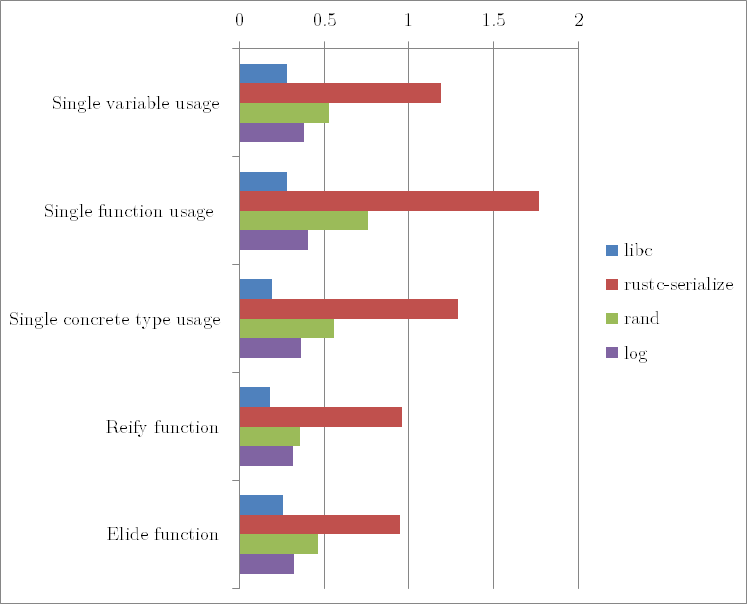
\includegraphics[width=8cm]{refactorings}

\caption{Graph displaying results of the different refactorings}
\label{Fig:compareref}
\end{center}
\end{figure}

\subsubsection{Varying the number of refactoring locations or usages}
From `libc', a number of different concrete types were targeted for performing a rename. `libc' was chosen for having a wider variety of occurrence counts specifically with concrete types. Figure \ref{Fig:comparerefs} shows how concrete type renaming appears to scale linearly (as expected from Chapter \ref{C:impl}) with the number of usages. Ideally, this analysis would have been done with other refactorings, but finding a reasonable amount of variation on the number of usages was difficult and searching was mostly manual. All the rename refactorings generally follow similar code paths and so the idea is that they should all scale in the same way (with the same general relationship). In particular, investigating function renaming would have been insightful as they take inherently more time. Although we expect to always scale linearly with the number of usages, the entire compiler is invoked each time instead of running what is actually necessary, like name resolution. As such, improvements can likely be made to the multiplying factor. As for the lifetime refactorings, the selection for the earlier timings did not strongly consider the number of visible `\&' and from observation, the time they took did not generally vary significantly. This is probably because they do not use additional passes of the compiler. Investigating scalability allows us to predict the time required for refactoring larger codebases. Referring back to Fowler, this is important for a tool since taking too long means that a programmer would simply prefer to do the refactoring by hand.

%In particular, Other crates or types of renamings had few examples and only a limited amount of variation.

\begin{figure}[h]
\begin{center}
    \begin{tabular}{ | l | c |}
    \hline
    \textbf{Number of replaced occurrences} & \textbf{Time in seconds} \\ \hline
    1 type usage &  0.1925  \\ \hline
    3 type usages &  0.3821  \\ \hline
    4 type usages &   0.4749  \\ \hline
    6 type usages &   0.6737  \\ \hline
    8 type usages &   0.8739 \\ \hline
    13 type usages  &  1.373 \\ \hline
    29 type usages &  2.960  \\ \hline
    51 type usages &  5.059 \\ \hline
    \end{tabular}
\end{center}

\caption{Timings for varying usage counts of concrete types in libc}
\label{Fig:scaling}
\end{figure}

\begin{figure}[h]
\begin{center}

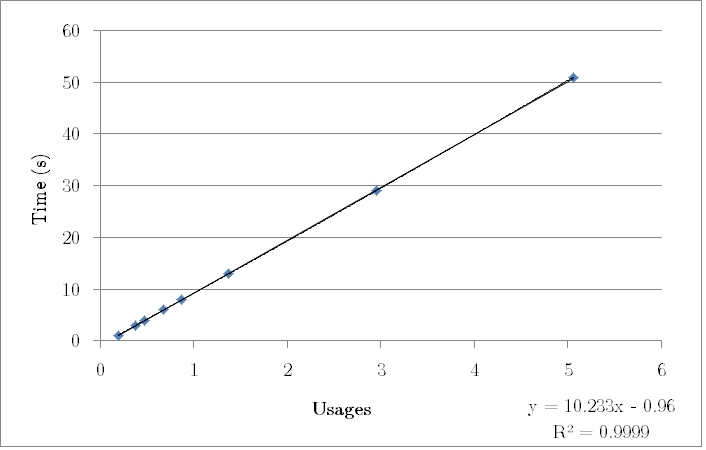
\includegraphics[width=8cm]{scaling}

\caption{Graph displaying results of varying the number of usages}
\label{Fig:comparerefs}
\end{center}
\end{figure}

Rust generally encourages the use of Crates.io and package management to form modular systems. This means that the amount of code implemented by you personally is as minimal as possible, making scalability potentially a non-issue. On the other hand, more modular systems mean more API and shared functions, types etc. While this might not affect performance it affects the overall difficulty of refactoring because once an API is exposed, it is usually not liable to change. Changes across different code-bases are problematic, not just for Rust, but for programmers in general (due to different owners, licenses, etc.).





\subsection{Other potential methods of evaluation} \label{S:otherstuff}
%The types of considerations which could have been done are as follows:
%Design considerations - well, workflow problems
Comparison to Eclipse or IntelliJ might have provided some useful points of contrast, but the language differences would make many of the comparisons difficult or meaningless. In particular, what is not immediately clear is how much correctness checking these tools actually perform. Eclipse could be investigated by looking at their codebase, but fundamentally Java is quite a different language to Rust with different complexities. There is also Rust specific refactorings here, but a notable point of comparison is definitely inlining. In downloading and installing a recent version of Eclipse, it appears that even the consideration of preventing an inline when the variable appears in a simple assignment was ignored.

A user study may have been another avenue to explore, but this appeared inappropriate for a number of reasons. We could bring in users of Rust, but the language is still in the process of gathering popularity. Finding those with the adequate amount of experience would likely be limited to those working heavily with the language, possibly working on the compiler (when our real target demographic is the casual user of Rust who does not know the inner workings well). There would also be few points of comparison, besides perhaps manual refactoring. A good deal of time was spent just determining what could even be done as part of this tool. Trying to juggle a user evaluation would have detracted from the goal of exploring the actual problems with a specifically Rust, refactoring tool. 

\section{Discussion}\label{C:future}

The work done so far serves as definite proof of the concept and the approaches used to build the refactoring tool. As explained by the evaluation, there is still work to be done to allow users to make the most out of the tool; both on this tool and more widely.

% The scope of this additional work extends far beyond the time allocated and should serve as an adequate starting point for those looking to extend this work in the future. At this point the goal of this work is to address immediate shortcomings in the tool and to leave the more complicated refactoring and infrastructure changes for others (while providing useful commentary and insight). Lastly, with Rust being an open source project, there is the issue of upstreaming code and being mindful of the fact that the tool should follow as many coding conventions as possible.

% DON'T FORGET to mention
% Contribution is about a dozen commits to the main compiler repository: https://github.com/rust-lang/rust/commits/master?author=gsam

\subsection{Future work on this tool}
\subsubsection{Wider project interaction}
% !!!!!!!!! TO INSERT !!!!!!!!!!!!!!!!!!!As of right now, allowing additional dependencies is managed by an environment variable which is neither robust or `safe' (due to the fact that changing this across threads for instance will likely cause negative consequences). Modifying the library API so that the calls have the additional dependencies handed to them appears desirable, however, slightly involved in any case.

One area of particular interest would be to investigate the overall effect of refactorings across multiple crates and how warnings (or patching scripts) should be presented when changes occur that might affect a public API. Examining the evaluation, this appears to be a major shortcoming in how not only this tool functions, but how other tools function across codebases. An investigation of Crates.io \cite{cratesio15}, the Rust package repository might yield interesting findings on crate interaction. One goal might be to describe the best steps to take when an API must change and how that should be dealt with from a community perspective. 

%Looking at how the UNIX/Linux community deals with API or ABI changes in their open source software should also prove useful.

\subsubsection{Testing and current test failures}
Going forward, the refactoring tool needs more testing to ensure that the current set of refactorings are correct. In adding functionality, tests ensure that existing refactorings are not broken with further changes to the tool. Furthermore, the refactoring tool evolves independently of the Rust compiler and changes to the compiler inevitably affect the outcome of the tool. Already, a number of existing compiler bugs have been found and reintroducing them by accident does not appear to be difficult with current limitations in the amount of testing and documentation available for some areas of the compiler. In this manner, expanding testing does not necessarily need to be confined to the refactoring tool. 

% At the moment, it has much less testing for multi-file. 

With limited experience with Rust in general, using real-world code to attempt refactorings would help test for more obscure corner cases which may have been overlooked. Some initial testing with Crates.io \cite{cratesio15} has been done along with initial analysis of its efficiency and usefulness, but more should be done in the future. 

%Furthermore, additional analysis of the efficiency of the tool can be produced and speculations made in regards to its usefulness. 

As of right now, the test cases identify roughly 10 incorrectly handled, but somewhat exceptional cases. A few of them likely require the addition of further investigation to determine their underlying source of error. On the other hand, a few of them are relatively subjective, in that they could be solved by simply restricting the inputs to the tool. One clear issue is that function local definitions currently cause name resolution issues. They appear to be at least solvable within the current tool architecture though. Elision is another source of failures, being only partly complete, having holes which were noted in Chapter \ref{C:impl}.
%  For instance, crate relative names break their current qualifications (further explanation?).  Furthermore, xxx.

\subsubsection{Future refactorings}
In terms of future refactorings, there are a number of next-step refactorings which should use most of the same infrastructure of the existing tool. For instance, trait renaming should use most of the same conventions provided by concrete types like structs or enums. This is because of the output of save-analysis and the simplifications made in process of generating the csv output. Renaming and modifying type aliases should present interesting problems due to deviations from typical object-orientated languages, along with type parameters and associated types. Furthermore, as previously described, renaming types declared within some function introduces issues to do with path resolution that still need to be resolved. To do so requires determining which parts of the path are `private' to that scope and should not be used in the general case. The treatment of types in Rust generally complicates matters, and this is already with the simplifications made from save-analysis.

In the context of Rust, there are a number of refactorings which would be more unique. Extraction of a method, as described by Fowler, presents a number of intricacies tied with lifetimes and the ownership system in Rust. Ensuring borrows are made correctly (or move semantics if a constructor is present in the extracted code) presents difficulties specific to Rust refactoring. While other refactoring changes are semantics preserving, extraction of a method could introduce new lifetimes and verification of correctness may not be so trivial. Similarly, extraction of local variables appears to provide difficulties with the ownership system and should be tackled first to provide insights for approaching method extraction.

Although not implemented here, inlining of functions was considered to some depth. Rust has the fortunate advantage of being able to evaluate a block of code as an expression, returning the result of the final line. This should allow relatively straightforward inlining of function bodies when there is a single return at the end, or no return at all. Where it becomes more complicated is with early returns whose control flow cannot be modelled simply by a block expression (which do not have the concept of early returns). This could normally be mitigated by the use of a labelled goto-like construct, however, Rust does not support goto which makes this a much more difficult problem. Whether or not classic gotos can even be implemented in Rust appears to be an open problem due to the marked increase in difficulty in static analysis (scoping or typing rules). There are labelled loop break-continue statements, so one approach might be to wrap the block in a loop. Further issues include redeclaration of arguments, or alternatively renaming of arguments and identifying when double nesting of blocks is required to achieve the correct scoping and lifetimes. 

Extraction, when compared to inlining, adds additional issues such as determining code-spans for expressions or the potential use of declared but uninitialized variables. In the standard case, extracting a local appears to be feasible as long as the same scope can be achieved; however, there is yet to be any actual evidence besides conjecture.

%Such a change is common with unstable API and within Rust, although released, there are a number of unstable API. 
Converting functions to methods or vice versa is also a critical function that would be useful for the Rust community. To alleviate issues with API changes, supporting these changes with a refactoring tool would be incredibly useful, even if it only used a structural search and replace. This would provide functionality similar to gofmt and go-fix as Go originally updated their API \cite{gofix11}. Making changes which break a sizable amount of user-code is unfavourable, however, it usually must be done at some point and having a tool to remedy the stress of such a change would be good for both the developers of Rust and the community. A non-comprehensive list of further refactorings to be considered are:

\begin{multicols}{2}
\begin{itemize}
\item Inlining methods
\itemsep0em 
\item Creating or inlining modules
\itemsep0em 
\item Adding or removing function args
\itemsep0em 
\item Changing types to type aliases
\itemsep0em 
\item Extracting traits or moving inherited to trait
\end{itemize}
\end{multicols}


% List a number of refactorings which would be interesting in the context of Rust
% Comparing closures to other languages
% Extract a global
% Constructor to factory?
% Unknown the extent to which refactoring works in unsafe code blocks

\subsubsection{Modularity of code}
While the evaluation mostly concerned external qualities of the tool, another aspect that could have been considered is the relative difficulty of adding or modifying refactorings. Currently, the compiler is tightly coupled with the refactoring tool and if you compare this to the Scala refactoring tool, you might find the latter uses much more well-established API and is more readily composable. In a similar way, JRRT likely benefits from the `obliviousness' of aspects \cite{aop}, being structured in such a way that injecting code is not noticed by the original program code. Whether this should be achieved here, or by working more with the compiler, it appears an important detail to enable wider contributions to the tool.


\subsection{Limitations in the performance evaluation}
Perhaps the most obvious shortcoming in these tests is the lack of sufficient data points, especially when trying to justify a trend. Finding the current set of examples was already extremely difficult given the size of the crates, made worse by the lack of macro support. Originally, a fifth crate `bitflags' was to be analyzed; however, the entire crate formed a macro expansion, preventing any refactoring. `libc' was almost entirely header declarations, having no `let' bindings, which made it difficult to generate the full set of refactorings. Performing scaling tests on more than just renaming types would have been helpful to prove worst-case linear scaling, especially for renaming functions as it was noticeably slower. But finding any meaningful variation of occurrences was difficult, and having but a few usages was common (as seen by the concentration of points in Figure \ref{Fig:comparerefs}). The relative size of the crates is still quite small and how the tool functions on much larger codebases is still completely unknown. Missing inline definitely limits the amount of useful conclusions that can be draw here. But the fact that few suitable locations for its usage were found questions the usefulness of the refactoring and the associated checks (given how incomplete they are). 

\subsection{Subjectivity in refactoring}
One of the reasons refactoring is not a straightforward topic is because of the different ways people might interpret a refactoring. In some domains or context, a perceivable behaviour violating change may not even matter. There are some cases where garnering user feedback will offer a clear-cut decision, but there are likely cases that will not. Caring is important because even if a user dislikes the way code is pretty-printed, for instance, they might avoid a tool entirely. Offering choice sounds good, but deciding what is an error, or a warning is still not easy (with better granularity here being a goal). One recent example that has come to light is the existence of conditional compilation within Rust. If performing a refactoring breaks other platforms, but not yours, should that be a problem? In particular, you may not have the required analysis of the remaining code, in which case a failure might be better.

\subsection{Missing formalisms}
As raised throughout this report, lack of formalism is an ongoing problem in the area of refactoring. General progress in the field of refactoring appears quite slow, with many opting to simply produce implementations rather than tackling the problem at large. In terms of missing formalisms, refactoring is not the only one at blame it appears. Much in the same way, compilers encode otherwise undescribed aspects of programming languages. Rust is no different, and the case with the relatively informal elision RFC (which was descriptive but definitely not complete) was a reminder of this. Being well-defined likely would have allowed reversal of the elision rules with much more ease. This is not a reason to point blame, but to highlight the genuine scale and complexity of the projects and issues at hand. 

%\subsection{Associated areas of work or research}
\subsection{Additional compiler improvements}
% -Z save-analysis
Given the current architecture of the tool, there are a number of further improvements that could be made to the compiler to improve its efficacy and efficiency. Using {\verb|-Zsave-analysis|} provides another additional step before a refactoring can be made. Furthermore, it must be generated every time a refactoring is to be undergone. By providing a library and API with which this information can be queried using the existing compiler API, the need for csv parsing and associated unrelated complexity disappears. The actual performance offset of having to run the compiler again to generate this information does not disappear however.  

%By running all the way through to analysis, this still takes a significant amount of time. 

%[reference to compiler stages from earlier section]

%  Compiler speed-up + Name resolution at the lowest level
Helping to address performance in the compiler itself in the general case should also help to improve performance of the refactoring tool. However, based on the current design of the tool and the need for multiple runs with modified source, the issue of performance would be better addressed by improvements to the name resolution module in the Rust compiler. In particular, providing name resolution for usages instead of just at the declaration level would turn O(N) runs of the compiler into O(1) by using name resolution multiple times in a single run. Fundamentally this requires heavy changes to the structure of the compiler and the nature of name resolution. As it currently is, not every node gets its individual node id in nested expressions and to resolve this requires significantly more memory usage or novel, significant and well-architected changes, well beyond the scope of this project.

% Macro hygiene with types
% Renaming within macros - seems like a big problem

Currently macros are completely ignored by the save-analysis report generated by the compiler. As it is, this appears to be a major shortcoming in the refactoring tool that has yet to be addressed. However, not a lot can be done at this point due to the general limitations regarding macros and how they are typically ignored when generating metadata from the compiler. Without being able to identify any spans associated with macros, it isn't possible to make the necessary code transformations. Implementing the necessary functionality is certainly non-trivial and likely requires much better domain knowledge than that which could be provided here. Resolving this would also fix pretty printer abstraction layer issues.

\subsection{Miscellaneous}

%[TODO: perhaps move somewhere else]
%A user-study or fielding comments on the tool would provide some interesting feedback. In order to provide usefulness, this is incredibly important part of assessing a tool. Furthermore production of a prototype GUI tool or Emacs plugin could increase the amount of users of the tool, or people interested in the tool. That could generate interest in further development and further research began by this project.

% Macro hygiene vs refactoring
The relationship between macro hygiene and refactoring is particularly novel, but from initial analysis, does not appear to provide any particular benefits. Further research into the relationship might provide some unique insights and a system which is able to incorporate both would be of significant academic interest, and interest to this author.

Efficiency of large-scale refactoring in general needs more attention. Although analysis of individual packages on a service like Crates.io provides some benefits, it would be curious to see how a tool functions on code bases which are much larger, in the order of hundreds of thousands of lines of code or larger. Although the expectations on this particular tool are not quite so high, understanding the general tradeoffs of provably correct refactorings and time taken and developer perception of this tradeoff is likely to produce fascinating observations. Looking at the Google-scale of refactoring, Google have set up a Clang map-reduce to perform refactoring on large codebases over a network of machines \cite{carruth2011clang}. Evidently the utility and associated confidence in such refactorings led them to spend the time to create such a framework, but determining when this happens in the general case provides provocative food-for-thought.


\section{Conclusion}\label{C:con}
% Documentation of API is necessary.
This work has explored refactoring and providing tool-support within the context of the Rust programming language. Utilizing existing infrastructure provided by the compiler, this work identifies extensions which help facilitate common automated refactorings. In a more general sense, this work attempts to build upon existing work done on refactoring by documenting specific decisions made in building a refactoring tool (which might normally only be encoded in the source code of an actual tool), and attempting to analyze the decisions made by others.

% Rust provides some unique obstacles in providing automated refactorings...

At the moment the provided tool supports renaming of local and global variables, fields, function arguments, structs, enum and functions (or methods). Beyond renaming, it also allows reification and elision of lifetime parameters for functions and methods and has preliminary support for inlining of local variables. These refactorings in particular highlight the idiosyncrasies of Rust, ensuring that the analyses performed here are some of the first of its kind. The complete limitations of these refactorings are not yet fully known, but there exists a current suite of tests to ensure that there are no obvious flaws in the approach. The presence of bugs in the compiler is a real problem to generality, but without real world use and more contribution to testing, finding these corner cases appears to be difficult.

At the moment, Rust lacks significant refactoring tool-support and evidently requires more work particularly within the compiler to enable further, valuable progress. Although a preliminary tool has been provided, there are many avenues for continuing work and the hope is that this first investigation provides useful insight for future efforts. Understanding the required context and the necessary infrastructure has been a major part of this work. In particular, learning and understanding Rust has been incredibly challenging, as it introduces concepts rarely used elsewhere. Continuation of this work should allow greater focus on implementing a more difficult and comprehensive set of refactorings for Rust.

\section{Appendix}\label{C:appen}
\section{Eclipse refactorings}
\begin{center}
\begin{figure}
\scalebox{0.9}{
\begin{tabular}{ l | l | l }
Rename &
Move &
Extract Method \\
Extract Local Variable &
Extract Constant &
Inline \\
Move Type to New File &
Extract Superclass &
Extract Interface \\
Push Down &
Pull Up &
Extract Class \\ 
Introduce Indirection &
Introduce Factory &
Introduce Parameter \\
Encapsulate Field &
Generalize Declared Type &
Migrate JAR File \\
Change Method Signature &
Convert Anon. Class to Nested &
Convert Local Variable to Field \\
Use Supertype Where Possible &
Introduce Parameter Object &
Infer Generic Type Arguments
\end{tabular}
}
\caption{List of refactorings supported by Eclipse}
\label{Fig:eclipse}
\end{figure}
\end{center}


%\section{Introduction}
%\label{intro}
%Your text comes here. Separate text sections with
%\section{Section title}
%\label{sec:1}
%Text with citations \cite{RefB} and \cite{RefJ}.
%\subsection{Subsection title}
%\label{sec:2}
%as required. Don't forget to give each section
%and subsection a unique label (see Sect.~\ref{sec:1}).
%\paragraph{Paragraph headings} Use paragraph headings as needed.
%\begin{equation}
%a^2+b^2=c^2
%\end{equation}

%% For one-column wide figures use
%\begin{figure}
%% Use the relevant command to insert your figure file.
%% For example, with the graphicx package use
%  \includegraphics{example.eps}
%% figure caption is below the figure
%\caption{Please write your figure caption here}
%\label{fig:1}       % Give a unique label
%\end{figure}
%%
%% For two-column wide figures use
%\begin{figure*}
%% Use the relevant command to insert your figure file.
%% For example, with the graphicx package use
%  \includegraphics[width=0.75\textwidth]{example.eps}
%% figure caption is below the figure
%\caption{Please write your figure caption here}
%\label{fig:2}       % Give a unique label
%\end{figure*}
%%
%% For tables use
%\begin{table}
%% table caption is above the table
%\caption{Please write your table caption here}
%\label{tab:1}       % Give a unique label
%% For LaTeX tables use
%\begin{tabular}{lll}
%\hline\noalign{\smallskip}
%first & second & third  \\
%\noalign{\smallskip}\hline\noalign{\smallskip}
%number & number & number \\
%number & number & number \\
%\noalign{\smallskip}\hline
%\end{tabular}
%\end{table}

%\begin{acknowledgements}
%If you'd like to thank anyone, place your comments here
%and remove the percent signs.
%\end{acknowledgements}

% BibTeX users please use one of
\bibliographystyle{spbasic}      % basic style, author-year citations
%\bibliographystyle{spmpsci}      % mathematics and physical sciences
%\bibliographystyle{spphys}       % APS-like style for physics
\bibliography{garming}   % name your BibTeX data base

\end{document}